\documentclass[a4paper,onecolumn,oneside,12pt,withmarginpar]{mwrep}
\usepackage{polski}
\usepackage{helvet}
\usepackage[T1]{fontenc}
\usepackage{anyfontsize}
\usepackage[utf8]{inputenc}
\usepackage[pdftex]{graphicx}
\usepackage{tabularx}
\usepackage{array}
\usepackage[polish]{babel}
\usepackage{subfigure}
%\usepackage{amssymb}
\usepackage{amsfonts}
\usepackage{gensymb}
\usepackage{verbatim}
\usepackage{indentfirst}
\usepackage[pdftex]{hyperref}
\usepackage{amsmath}
\usepackage{float}
%\usepackage{fancyheader} % nagłówek i stopka

\usepackage{xargs}                      % Use more than one optional parameter in a new commands
\usepackage[pdftex,dvipsnames]{xcolor}  % Coloured text etc.

\usepackage[colorinlistoftodos,prependcaption]{todonotes}

\newcommandx{\unsure}[2][1=]{\todo[linecolor=red,backgroundcolor=red!25,bordercolor=red,#1]{#2}}
\newcommandx{\change}[2][1=]{\todo[linecolor=blue,backgroundcolor=blue!25,bordercolor=blue,#1]{#2}}
\newcommandx{\improve}[2][1=]{\todo[linecolor=Plum,backgroundcolor=Plum!25,bordercolor=Plum,#1]{#2}}

% kursywa dla słów anglojęzycznych
\newcommand{\ang}[1]{\textit{#1}}


\usepackage{enumitem}
\setlist{nolistsep}

\hyphenpenalty=10000		% nie dziel wyrazów zbyt często
\clubpenalty=10000			% kara za sierotki
\widowpenalty=10000			% nie pozostawiaj wdów
\brokenpenalty=10000		% nie dziel wyrazów między stronami
\exhyphenpenalty=999999		% nie dziel słów z myślnikiem
\righthyphenmin=3			% dziel minimum 3 litery


\tolerance=4500
\pretolerance=250
\hfuzz=1.5pt
\hbadness=1450
\sloppy						% umacnia pozycję prawego marginesu

\renewcommand*{\figurename}{Rys.} 
\renewcommand*{\tablename}{Tab.} 


% na oprawe (1.0cm - 0.7cm)*2 = 0.6cm
% na oprawe (1.1cm - 0.7cm)*2 = 0.8cm
%  oddsidemargin lewy margines na nieparzystych stronach
% evensidemargin lewy margines na parzystych stronach

%ILE MA MIEĆ OPRAWA??
\def\oprawa{1.05cm}
\addtolength{\oddsidemargin}{\oprawa}
\addtolength{\evensidemargin}{-\oprawa}

% table span multirows
\usepackage{multirow}

%\setlist{listparindent=\parindent, parsep=\parskip} % potrzebuje enumitem


%%%%%%%%%%%%%%% Dodatkowe Pakiety %%%%%%%%%%%%%%%%%
\usepackage{prmag2017}   % definiuje komendy opiekun,nrindeksu, rodzaj pracy, ...


%%%%%%%%%%%%%%% Strona Tytułowa %%%%%%%%%%%%%%%%%
% To trzeba wypelnic swoimi danymi
\title{Raspberry Pi jako zoptymalizowany pod względem kosztu sieciowy system akwizycji danych}

% autor
\author{Krzysztof Wasilewski}
\nrindeksu{265956}

\opiekun{dr inż. Wojciech Zabołotny}

\terminwykonania{28 stycznia 2018} % data na oświadczeniu o samodzielności
\rok{2018}


% Podziekowanie - opcjonalne
%\podziekowania{\noindent
{\Large Podziękowania}
\bigskip

Dziękuję bardzo serdecznie wszystkim, a w szczególności rodzicom i promotorowi.

\bigskip

{\raggedleft
Krzysztof Wasilewski

}

}

\miasto{Warszawa}
\uczelnia{POLITECHNIKA WARSZAWSKA}
\wydzial{WYDZIAŁ ELEKTRONIKI
\linebreak[1] I TECHNIK INFORMACYJNYCH}
\instytut{Instytut Systemów Elektronicznych}
\zaklad{Zakład Układów i Systemów Elektronicznych}
\kierunekstudiow{Elektronika}
\specjalnosc{Elektronika i Inżynieria Komputerowa}

%%% koniec od P.W

\opinie{%
  \newpage
\begin{center}
 {\large\bf  Opinia} \\
o pracy dyplomowej magisterskiej wykonanej przez dyplomanta\\
{\bf Zdolnego Studenta i Pracowitego Kolegę} \\
 Wydział Elektryczny, kierunek Informatyka,  Politechnika Warszawska\\
Temat pracy\\
\textit{\bf
TYTUŁ PRACY DYPLOMOWEJ
}\\
\end{center}
\medskip
\noindent
Promotor: {\bf dr inż. Miły Opiekun}\\
Ocena pracy dyplomowej: {\bf bardzo dobry}

\medskip

\centerline{\bf Treść opinii}
   Celem pracy dyplomowej panów dolnego Studenta i Pracowitego Kolegi  było
opracowanie systemu pozwalającego symulować  i opartego o oprogramowanie o
otwartych źródłach (ang. Open Source). Jak piszą Dyplomanci, starali się opracować
system, który łatwo będzie dostosować do zmieniających się dynamicznie wymagań,
będzie miał niewielkie wymagania sprzętowe i umożliwiał dalszą łatwą rozbudowę oraz
dostosowanie go do potrzeb.
Przedstawiona do recenzji praca składa się z krótkiego wstępu jasno i
wyczerpująco opisującego oraz uzasadniającego cel pracy, trzech rozdziałów (2-4)
zawierających opis istniejących podobnych
rozwiązań, komponentów rozpatrywanychjako kandydaci do
tworzonego systemu i wreszcie zagadnień wydajności wirtualnych
rozwiązań. Piąty rozdział to opis przygotowanego przez
Dyplomantów środowiska obejmujący opis konfiguracji
środowiska oraz przykładowe ćwiczenia laboratoryjne. Ostatni
rozdział pracy to opis możliwości dalszego
rozwoju projektu. W ramach przygotowania pracy Dyplomanci zebrali i przedstawili w
bardzo przejrzysty sposób duży zasób informacji, co świadczy o dobrej orientacji
w nowoczesnej i ciągle intensywnie rozwijanej tematyce stanowiącej
zakres pracy i o umiejętności przejrzystego przedstawienia tych
wyników. Praca zawiera dwa dodatki, z których pierwszy obejmuje wyniki
eksperymentów i badań nad wydajnością, a drugi to źródła
skryptów budujących środowisko.

 Dyplomanci dość
dobrze zrealizowali postawione przed nimi zadanie,
wykazali się więc umiejętnością zastosowania w praktyce wiedzy
przedstawionej w rozdziałach 2-4.  Uważam, że cele postawione w założeniach pracy zostały pomyślnie
zrealizowane. Proponuję ocenę bardzo dobrą (5).

\vskip 1cm
{
\raggedleft
(data, podpis)\kern1cm

}
  \newpage
  \newpage
\begin{center}
 {\large\bf  Recenzja } \\
pracy dyplomowej inżynierskiej wykonanej przez dyplomanta\\
{\bf Krzysztofa Wasilewskiego} \\
 Wydział Elektroniki, kierunek Elektronika,  Politechnika Warszawska\\
Temat pracy\\
\textit{\bf
TYTUŁ PRACY DYPLOMOWEJ
}\\
\end{center}
\medskip
\noindent
Recenzent: {\bf prof. nzw. dr hab. inż. Jan Surowy}\\
Ocena pracy dyplomowej: {\bf bardzo dobry}
\medskip


\centerline{\bf Treść recenzji}
   Celem pracy dyplomowej panów dolnego Studenta i Pracowitego Kolegi  było
opracowanie systemu pozwalającego symulować  i opartego o oprogramowanie o
otwartych źródłach (ang. Open Source). Jak piszą Dyplomanci, starali się opracować
system, który łatwo będzie dostosować do zmieniających się dynamicznie wymagań,
będzie miał niewielkie wymagania sprzętowe i umożliwiał dalszą łatwą rozbudowę oraz
dostosowanie go do potrzeb.
Przedstawiona do recenzji praca składa się z krótkiego wstępu jasno i
wyczerpująco opisującego oraz uzasadniającego cel pracy, trzech rozdziałów (2-4)
zawierających bardzo solidny i przejrzysty opis: istniejących podobnych
rozwiązań (rozdz. 2), komponentów rozpatrywanychjako kandydaci do
tworzonego systemu (rozdz. 3) i wreszcie zagadnień wydajności wirtualnych
rozwiązań, zwłaszcza w kontekście współpracy  kilku elementów
 sieci (rozdział 4). Piąty rozdział to opis przygotowanego przez
Dyplomantów środowiska obejmujący opis konfiguracji
środowiska oraz przykładowe ćwiczenia laboratoryjne (5 ćwiczeń). Ostatni, szósty
rozdział pracy to krótkie zakończenie, które wylicza także możliwości dalszego
rozwoju projektu. W ramach przygotowania pracy Dyplomanci zebrali i przedstawili w
bardzo przejrzysty sposób duży zasób informacji o narzędziach, Rozdziały 2, 3 i 4 świadczą o dobrej orientacji
w nowoczesnej i ciągle intensywnie rozwijanej tematyce stanowiącej
zakres pracy i o umiejętności syntetycznego, przejrzystego przedstawienia tych
wyników. Drobne  mankamenty tej części pracy to zbyt skrótowe omawianie
niektórych zagadnień technicznych, zakładające dużą początkową wiedzę czytelnika
i dość niestaranne podejście do powołań na źródła.
Utrudnia to w pewnym stopniu czytanie pracy i zmniejsza jej wartość dydaktyczną
(a ta zdaje się być jednym z celów Autorów), ale jest zrekompensowane zawartością
merytoryczną. Praca zawiera dwa dodatki, z których pierwszy obejmuje wyniki
eksperymentów i badań nad wydajnością, a drugi to źródła
skryptów budujących środowisko. Praca
zawiera niestety dość dużą liczbę drobnych błędów redakcyjnych, ale nie wpływają
one w sposób istotny na na jej czytelność i wartość. W całej pracy przewijają
się samodzielne, zdecydowane wnioski Autorów, które są wynikiem własnych i
oryginalnych badań.  Rozdział 5 i dodatki pracy przekonują mnie, że Dyplomanci dość
dobrze zrealizowali postawione przed nimi zadanie. Pozwala to stwierdzić, że
wykazali się więc także umiejętnością zastosowania w praktyce wiedzy
przedstawionej w rozdziałach 2-4. Kończący pracę rozdział szósty świadczy o
dużym (ale moim zdaniem uzasadnionym) poczuciu własnej wartości i jest
świadectwem własnego, oryginalnego spojrzenia na tematykę przedstawioną w pracy
dyplomowej. Uważam, że cele postawione w założeniach pracy zostały pomyślnie
zrealizowane. Proponuję ocenę bardzo dobrą (5).

\vskip 1cm
{
\raggedleft
(data, podpis)\kern1cm

}
}
\streszczenia{
%\begin{center}
  \newpage
\begin{center}
\large \bf
Raspberry Pi jako zoptymalizowany pod względem kosztu sieciowy system akwizycji danych
\end{center}

\section*{Streszczenie}

Praca zawiera opis projektu i implementacji sieciowego systemu akwizycji danych z wykorzystaniem platformy Raspberry Pi. Głównym celem projektu było stworzenie systemu umożliwiającego użytkownikowi akwizycję danych pomiarowych i zachowanie jak najdokładniejszej, w granicach możliwości technicznych, informacji o czasie zebrania próbki. Podstawowym problemem w trakcie projektu było zapewnienie wykonania krytycznych czasowo zadań w wielowątkowym systemie operacyjnym Linux. W pracy przedstawione są możliwości różnych rozwiązań programowych. Projekt zakładał, że użytkownik będzie w stanie ustawiać parametry pomiarów zdalnie za pomocą aplikacji internetowej. Dodatkowymi założeniami były optymalizacja pod względem kosztu i łatwa rozszerzalność projektu. W piątym rozdziale zawarto opis testów sprzętu oraz testów funkcjonalnych i prezentację wyników. Ostatnią częścią pracy jest podsumowanie wraz z ukazaniem dalszych możliwości rozwoju projektu.

\bigskip
{\noindent\bf Słowa kluczowe:} system akwizycji danych, Raspberry Pi, sieć

\clearpage
\setcounter{page}{1}
\mbox{}

\clearpage


%\vskip 2cm
\newpage

\begin{center}
\large \bf
Raspberry Pi as a cost-optized network data aquisition system
\end{center}

\section*{Abstract}
Thesis includes project description of the network data aquisition system using Raspberry Pi platform. The main aim of the project was to build a system which can be used to aquisite data and save as much as possible accurate information about meassurement timestamp. The main issue was to ensure finishing time-critical tasks in multithreading Linux operating system. Thesis describes variety of software solutions to the problem. Project assumed that the user should be able to control the system via Web application. Another assumption was cost optimazation and developability of the project. In the fifth chapter hardware tests, functional tests and results summary are described.
The last part of the thesis is the assumption with capabities for futher development.

\bigskip
{\noindent\bf Keywords:} data aquisition system, Raspberry Pi, netowrk

\clearpage
\mbox{}
\clearpage

\vfill
%\end{center}
}

\begin{document}
\maketitle

\chapter{Wstęp}
\label{wstep}

\section{Wprowadzenie}

W dzisiejszych czasach w dobie Internetu i rozwoju Internetu Rzeczy rośnie zapotrzebowanie na wydajne i zoptymalizowane pod względem kosztu sieciowe systemy akwizycji danych. Rozwój technologii pozwolił na miniaturyzację czujników oraz zmniejszenie kosztu urządzeń zbierających dane pomiarowe.

Akwizycja (zbieranie) danych jest pierwszym i bardzo ważnym etapem przetwarzania danych, gdyż jakość systemu akwizycji wpływa na wydajność i dokładność całego systemu pomiarowego. Istotnym aspektem jest, by odpowiednio dobrać parametry techniczne systemu do konkretnego zastosowania, uwzględniając rodzaj transmisji, poziomy napięć logicznych czy wydajność prądową układu zasilania. 
Dodatkowo system sieciowy musi używać odpowiedniego do danego zastosowania protokołu transmisji.  

Główny nacisk pracy dyplomowej był położony na zachowanie jak najdokładniejszej informacji o czasie pomiaru i okresie próbkowania. Dodatkowo system powinien być zoptymalizowany pod względem kosztu. Użycie platformy Raspberry Pi daje dosyć duże możliwości, jednak ma też swoje ograniczenia. Pierwszym i jednocześnie największym sprzętowym ograniczeniem, wynikającym z zastosowania tej platformy jest brak przetwornika analogowo-cyfrowego na płytce. W celu obsługi sygnałów analogowych konieczne jest zastosowanie zewnętrznego układu. Parametry techniczne płytki Raspberry Pi oraz interfejsy wymiany danych jakie posiada pozwalają na podłączenie i pracę wielu układów peryferyjnych jednocześnie.


\section{Cel i zakres pracy}
Celem pracy było wykonanie zoptymalizowanego pod względem kosztu sieciowego systemu akwizycji danych z wykorzystaniem platformy Raspberry Pi. Projekt zakładał stworzenie płytki pomiarowej będącej rozszerzeniem do platformy Raspberry Pi umożliwiającej zbieranie danych z zewnętrznych urządzeń przy pomocy dostępnych interfejsów SPI i I$^2$C. Płytka powinna zawierać układy umożliwiające doprowadzenie sygnałów z zewnętrznych czujników. 
Sieciowy system akwizycji danych może być wykorzystany do stworzenia stacji meteorologicznej z funkcją zdalnego dostępu, możliwością sterowania i wyzwalania pomiarów oraz odbioru danych przez interfejs sieciowy.
\newpage
W zakres pracy wchodziło:
\begin{itemize}
\item Opracowanie sterowników jądra i aplikacji użytkownika umożliwiających obsługę przetworników i czujników pomiarowych podłączonych do komputera przez typowe interfejsy sprzętowe, takie jak I$^2$C, SPI
\item Zapewnienie akwizycji danych z zachowaniem jak najpełniejszej (w granicach możliwości technicznych) informacji o czasie pomiaru, w celu umożliwienia późniejszej analizy off-line danych z różnych źródeł z uwzględnieniem korelacji czasowej.
\item Przygotowanie serwerów i/lub programów klienckich umożliwiających udostępnienie zmierzonych danych przez sieć TCP/IP.
\item Realizacja interfejsu pozwalającego na zdalne sterowanie procesem pomiaru.
\end{itemize}

\bigskip

Podstawowym celem projektu było zaprojektowanie i realizacja systemu umożliwiającego użytkownikowi akwizycję danych pomiarowych, z zachowaniem jak najdokładniejszej informacji o znaczniku czasu w momencie zebrania próbki. W wielozadaniowym systemie operacyjnym zastosowanie aplikacji z przestrzeni użytkownika nie daje pewności co do reżimu czasowego wykonania poleceń zawartych w kodzie programu. W przypadku akwizycji danych z zewnętrznych przetworników podłączonych przez magistralę interfejsu szeregowego (np. \ang{spidev} dla interfejsu SPI) informacja o znaczniku czasu zarejestrowana w aplikacji z przestrzeni użytkownika nie jest dokładna i powoduje powstanie nieregularności okresu próbkowania.
W celu zapisania jak najdokładniejszej informacji o czasie pomiaru należy znacznik czasu pobrania próbki zarejestrować w przestrzeni jądra systemu.

W pracy przedstawione są możliwości różnych rozwiązań programowych. Niski koszt zbudowania systemu oraz łatwość rozszerzenia funkcjonalności powodują, że urządzenie stanowi konkurencję dla systemów komercyjnych. Projekt zakładał, że użytkownik będzie w stanie ustawiać parametry pomiarów zdalnie za pomocą aplikacji w przeglądarce internetowej. Dodatkowymi założeniami były optymalizacja pod względem kosztu i łatwa rozszerzalność systemu. W końcowej części pracy zawarto przebieg testów sprzętu oraz testów funkcjonalnych i podsumowanie wyników. 

\section{Układ pracy}
Praca została podzielona na sześć rozdziałów. Po niniejszym rozdziale wstępnym, w Rozdziale \ref{ch:zalozenia} dokonano przeglądu systemów akwizycji danych, przedstawiono założenia i wymagania postawione dla sieciowego systemu akwizycji danych oraz dla oprogramowania umożliwiającego obsłużenie urządzeń dołączanych do platformy Raspberry Pi.
W Rozdziale \ref{ch:projekt} przedstawiono projekt układu pozwalającego na realizację zaprojektowanego systemu akwizycji danych. Rozdział \ref{ch:soft} zawiera opis różnych rozwiązań programowych.
W Rozdziale \ref{ch:testy} przedstawiony jest przebieg oraz wyniki testów systemu. W Rozdziale \ref{ch:podsumowanie} zawarto podsumowanie projektu.


\chapter{Założenia}

\label{ch:zalozenia}

\section{Przykłady systemów akwizycji danych}

Na rynku jest dostępna szeroka gama systemów akwizycji danych. Większość dostępnych rozwiązań to układy do profesjonalnych zastosowań laboratoryjnych. Często urządzenia te pracują tylko pod określonym oprogramowaniem co zwiększa koszty. Powoduje to, że brakuje urządzeń, które posiadałyby podstawową funkcjonalność systemu akwizycji danych za cenę mniejszą niż 500zł. 

\subsection{System akwizycji danych NI USB6008}

Przykładem jest system akwizycji danych National Instruments USB6008. Urządzenie posiada 8 analogowych wejść i obsługuje interfejs USB. Zawiera 12-bitowy przetwornik analogowo-cyfrowy próbkujący z częstotliwością 10kS/s.\cite{NI_6008} Urządzenie kosztuje około 1000zł w celu wykonania pomiarów potrzebujemy komputera z zainstalowanym oprogramowaniem producenta, co powoduje generowanie dodatkowych kosztów.

\begin{figure}[h]
	\centering
		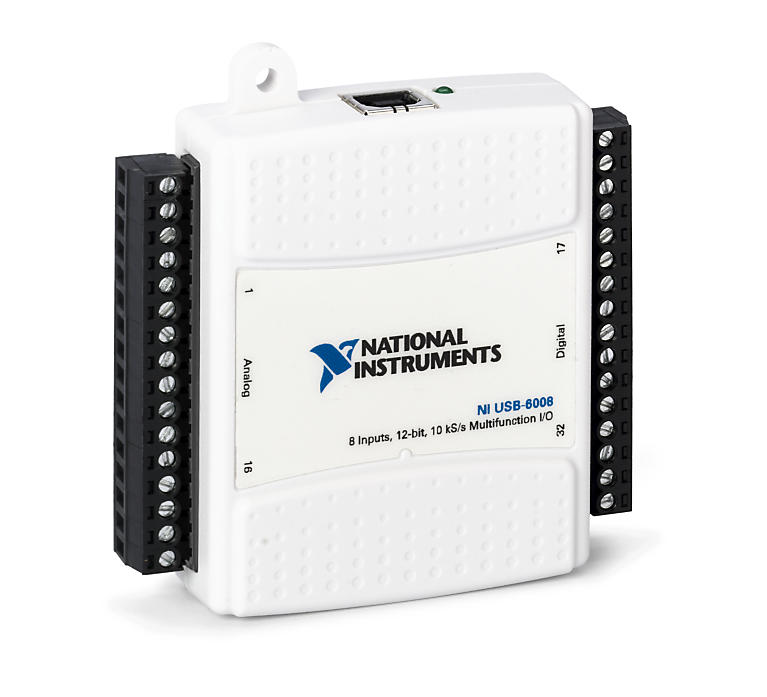
\includegraphics[width=10cm]{daq_ni_usb6008}
	\caption{National Instruments USB6008} 
	\label{fig:uxtouch}
\end{figure}

\subsection{Oscyloskop cyfrowy Digilent Analog Discovery 2}

Kolejnym przykładem systemu akwizycji danych jest przystawka do komputera osobistego  Digilent Analog Discovery 2. Urządzenie po podłączeniu do komputera PC oraz doprowadzeniu badanych sygnałów do jego wejść umożliwia wykonywanie pomiarów. Posiada następujące parametry techniczne\cite{AnalogDiscoveryDoc}

\begin{itemize}
\item 16-kanałowy analizator logiczny (14-bit, 100MS/s, +-5V) 
\item 2-kanałowy oscyloskop cyfrowy (14-bitowy, 100MS/s, +-25V) 
\item wzmacniacz audio-stereo, 
\item interfejsy SPI, I$^2$C, UART, USB
\item zasilanie 5V
\end{itemize}

\begin{figure}[h]
	\centering
		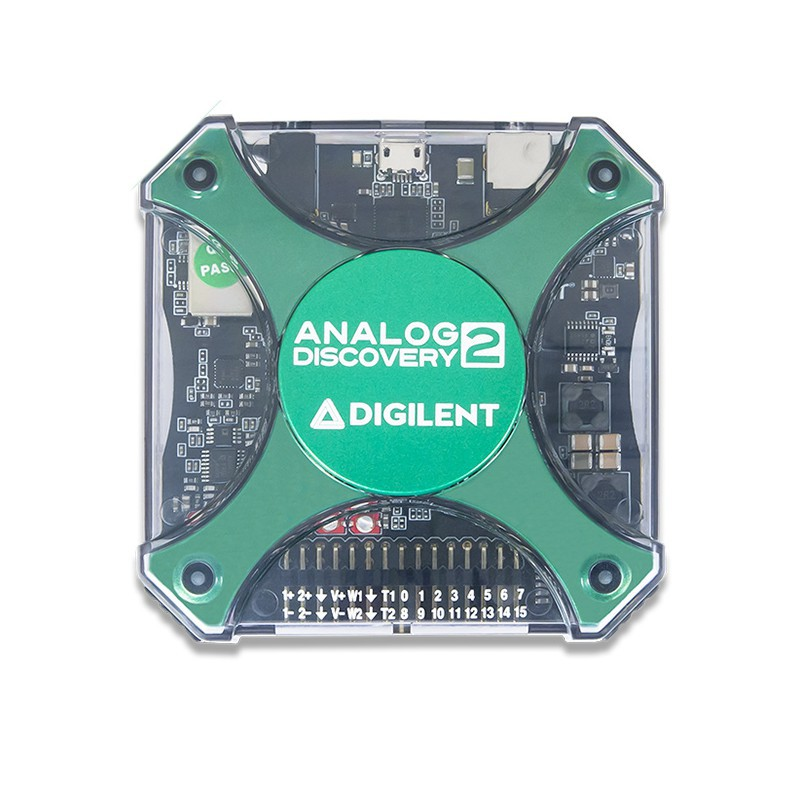
\includegraphics[width=10cm]{analog_discovery2}
	\caption{Digilent Analog Discovery 2} 
	\label{fig:uxtouch}
\end{figure}


Cena urządzenia jest zbliżona do poprzedniego przykładu (ok. 1000-1400zł), jednak oprogramowanie, pozwalające na pracę z przystawką jest darmowe, co znacząco obniża koszt całego systemu. Nie mniej jednak sama przystawka Digilent Analog Discovery 2 nie tworzy w pełni funkcjonalnego systemu akwizycji danych. Do poprawnego działania systemu potrzebny jest komputer osobisty z zainstalowanym dedykowanym oprogramowaniem.

Powyższe urządzenia nie posiadają interfejsu sieciowego. Zapewniają jedynie możliwość akwizycji danych na podłączonym przez port USB komputerze.

\section{Cechy systemu}
System powinien udostępniać możliwość obsługi sygnałów zarówno cyfrowych jak i analogowych. Ze względu na brak przetwornika analogowo-cyfrowego na płytce Raspberry Pi, konieczne jest użycie zewnętrznego układu.
Raspberry Pi może działać pod systemem operacyjnym Linux, który nie jest systemem czasu rzeczywistego, co powoduje, że w domyślnej konfiguracji systemu nie da się zagwarantować stałego odstępu czasowego pomiędzy odbieraniem próbek kolejnych z przetwornika. W celu wydajnego przetwarzania sygnałów większej częstotliwości dodano moduł do jądra systemu, zawierający implementację licznika wysokiej rozdzielczości, co powoduje zmniejszenie wahań częstotliwości próbkowania w trakcie pomiarów oraz pozwala na zachowanie momentu otrzymania próbki z dużą dokładnością.

\subsection{Informacja o czasie pomiaru}

Raspberry Pi jest komputerem zoptymalizowanym pod względem kosztów i rozmiaru, co sprawia, że jest pozbawiony podzespołów, które są zbyt drogie lub zajmują zbyt dużo miejsca na płytce. Jednym z takich układów jest układ RTC (z ang. Real Time Clock - zegar czasu rzeczywistego) Układ ten jest zasilany z baterii niezależnie od komputera i zapewnia przechowywanie czasu rzeczywistego po odłączeniu zasilania. 

System akwizycji danych powinien zapewniać w miarę możliwości technicznych jak najdokładniejszą informację o czasie zebrania próbki danych.
Raspberry Pi za pomocą protokołu NTP (z ang. Network Time Protocol - Sieciowy Protokół Czasu) jest w stanie synchronizować czas w systemie do wybranego w konfiguracji protokołu serwera. Korzystając z odpowiednich serwerów, NTP jest w stanie dostosować czas systemu klienta, uwzględniając opóźnienia w transmisji danych. Protokół posiada jednak ograniczoną dokładność spowodowaną

Wykorzystanie własnego sterownika do pomiaru napięcia przetwornika analogowo-cyfrowego pozwala na zebranie znacznika czasu z rozdzielczością pojedynczych nanosekund. 

\subsection{Zegar czasu rzeczywistego}

W przypadku, wykorzystania Raspberry Pi do pracy z ograniczonym dostępem do sieci warto dołączyć moduł zegara czasu rzeczywistego.
Istnieje możliwość rozszerzenia systemu o moduł RTC . Na rynku są dostępne moduły obsługiwane za pomocą interfejsów szeregowych SPI lub I2C. Jednym z najbardziej popularnych modułów zegara czasu rzeczywistego kompatybilnych z Raspberry Pi jest moduł z układem DS3231\cite{rtc}. Układ zawiera niezależne zasilanie bateryjne i działa po odłączeniu Raspberry Pi od źródła napięcia.
Moduł RTC z zasilaniem bateryjnym przedstawiono na Rys. \ref{pic:rtc}. 

\begin{figure}[h]
	\centering
		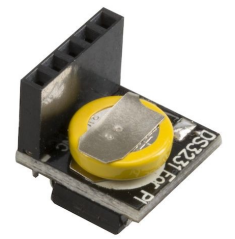
\includegraphics[width=5cm]{rtc}
	\caption{Moduł zegara czasu rzeczywistego z układem DS2331} 
	\label{pic:rtc}
\end{figure}

\section{Struktura systemu}

System składa się z platformy Raspberry Pi używanej jako komputer główny oraz dołączanej płytki pomiarowej umożliwiającej podłączenie czujników z możliwością łatwego doprowadzenia zasilania do wszystkich urządzeń. Platforma Raspberry Pi zapewnia w systemie kontrolę pomiarów i pozwala na wizualizację oraz udostępnianie otrzymanych wyników. 


\begin{figure}[h]
	\centering
		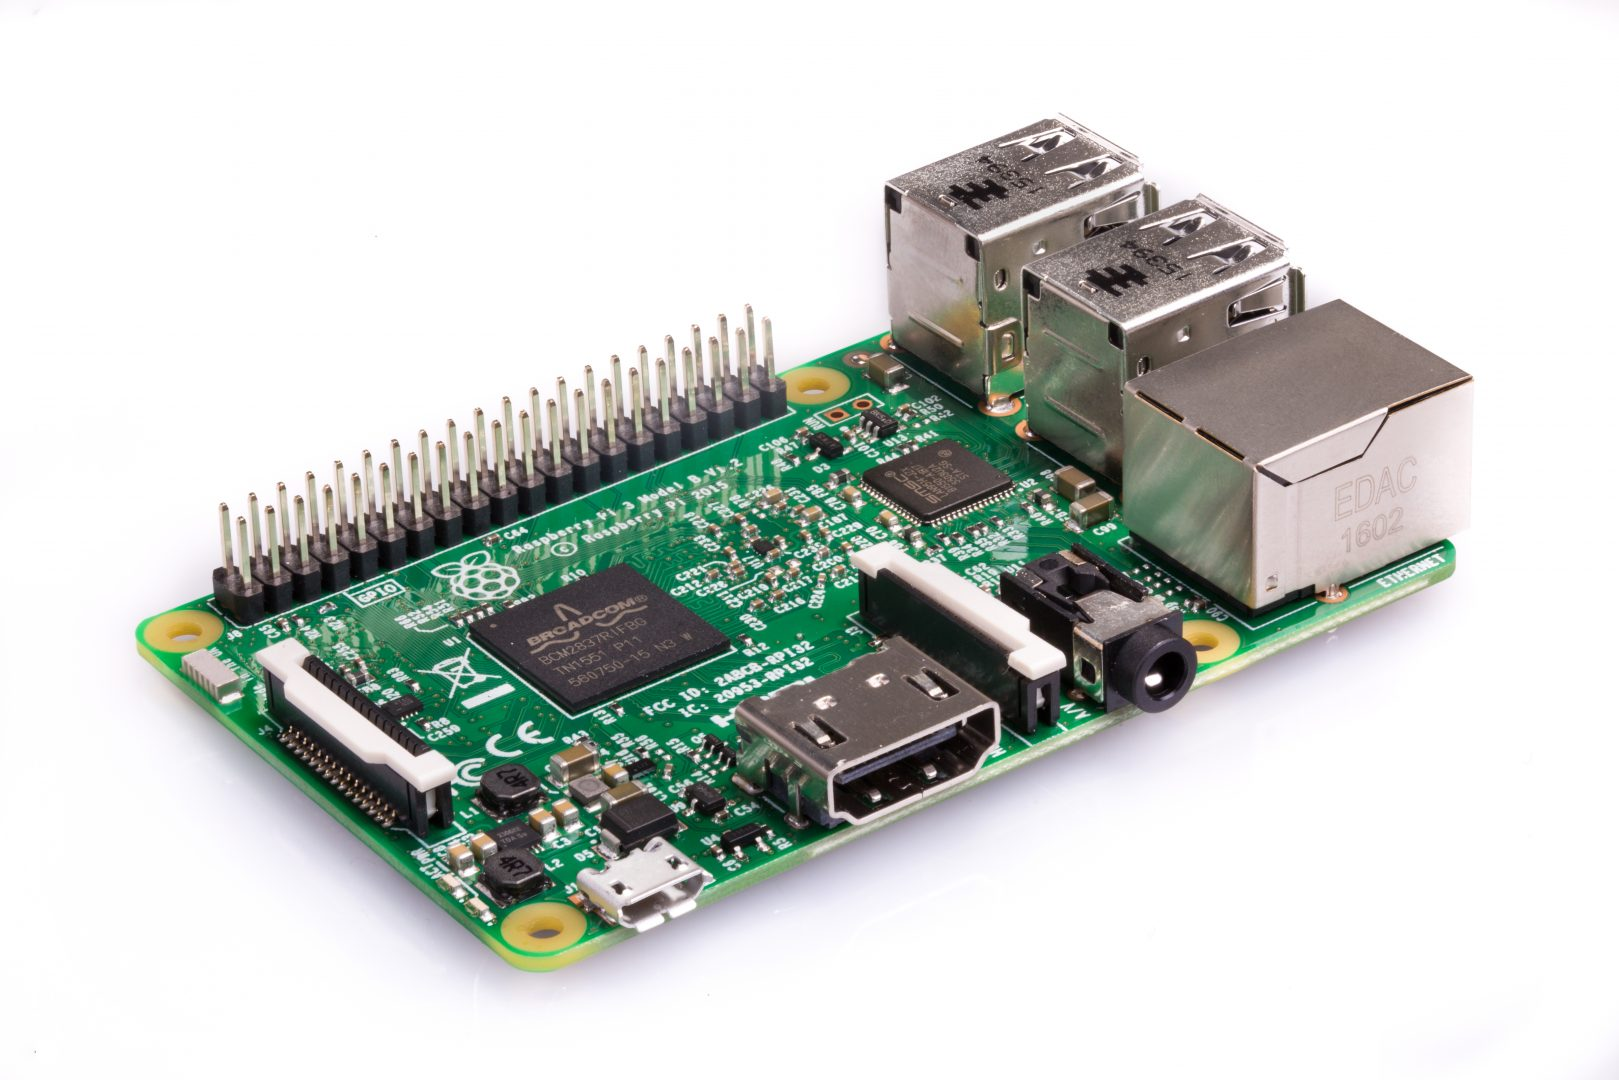
\includegraphics[width=14cm]{rpi}
	\caption{Raspberry Pi 3 Model B} 
	\label{pic:RPi}
\end{figure}

\subsection{Platforma Raspberry Pi}

Raspberry Pi to jednopłytkowa platforma stworzona przez Raspberry Pi Foundation. Pierwsza wersja minikomputera powstała w roku 2012 i była oparta o układ firmy Broadcom BCM2835 SoC (z ang. System on Chip - System wbudowany) oraz procesor graficzny Broadcom VideoCore IV. Głównymi zaletami platformy były niska cena w stosunku do możliwości.

Rozważano zastosowanie w pracy jednej z trzech wersji płytki:
\begin{itemize}
\item Raspberry Pi ZeroW
\item Raspberry Pi 2 Model B
\item Raspberry Pi 3 Model B, 
\end{itemize}

\begin{table}[t]
\label{tabRpi}
\centering
\begin{tabular}{|l|l|l|l|}
  \hline 
  Wersja płytki & ZeroW & 2 Model B & 3 Model B\\
  \hline
  Procesor CPU & 1GHz ARM1176JZF-S & 1,2 GHz ARM Cortex-A53 &  900 MHz \\
  \hline
  Pamięć RAM  512 MB & 1GB & 1 GB LPDDR2 &\\
  \hline
 Połączenia sieciowe & 10/100 Ethernet, Wi-Fi (2,4 GHz 802.11n) \\
  \hline

\end{tabular}
\caption{Parametry techniczne platformy Raspberry Pi 3 Model B 
\cite{rpispecs}
} 
\end{table}

Ze względu na małe różnice w cenie i założenie zastosowania bezprzewodowego dostępu do sieci zrezygnowano z wersji Model 2 B. Rozważano zastosowanie wersji ZeroW, która jest cenowo konkurencyjna do wersji Model 3 B i pozwala na bezprzewodowy dostęp do sieci za pomocą łącza Wi-Fi. Z powodu założenia przetwarzania dużej ilości danych przez system oraz współbieżnego wykonywania aplikacji równocześnie z obsługą interfejsów sieciowych wybrano wersję Model 3B.

 
Platforma Raspberry Pi w wersji 3 posiada liczne złącza m.in.: HDMI, Ethernet, 4 porty USB 2.0, wyjście 3,5mm jack, złącze kart microSD oraz 40-pinowe złącze GPIO. W tabeli poniżej przedstawiono specyfikacje wersji płytki użytej w projekcie - Raspberry Pi 3 Mdel B:

\begin{table}[t]
\label{tabRpi}
\centering
\begin{tabular}{|l|l|l|}
  \hline 
  Nazwa układu SoC & Broadcom BCM2837 \\
  \hline
  Procesor CPU & 1,2 GHz quad-core ARM Cortex-A53 (64-bit) \\
  \hline
 Procesor graficzny GPU & Broadcom VideoCore IV \\ 
  \hline 
  Pamięć RAM  & 1 GB LPDDR2 (900 MHz) \\
  \hline
 Napięcie zasilania & 5 V, złącze MicroUSB lub GPIO\\
  \hline
 Połączenia sieciowe & 10/100 Ethernet, Wi-Fi (2,4 GHz 802.11n) \\
  \hline
 Nośnik danych  & złącze kart MicroSD \\
 \hline
 Interfejsy szeregowe & SPI, I$^2$C, UART \\ 
  \hline
\end{tabular}
\caption{Parametry techniczne platformy Raspberry Pi 3 Model B 
\cite{rpispecs}
} 
\end{table}

\begin{figure}[h]
	\centering
		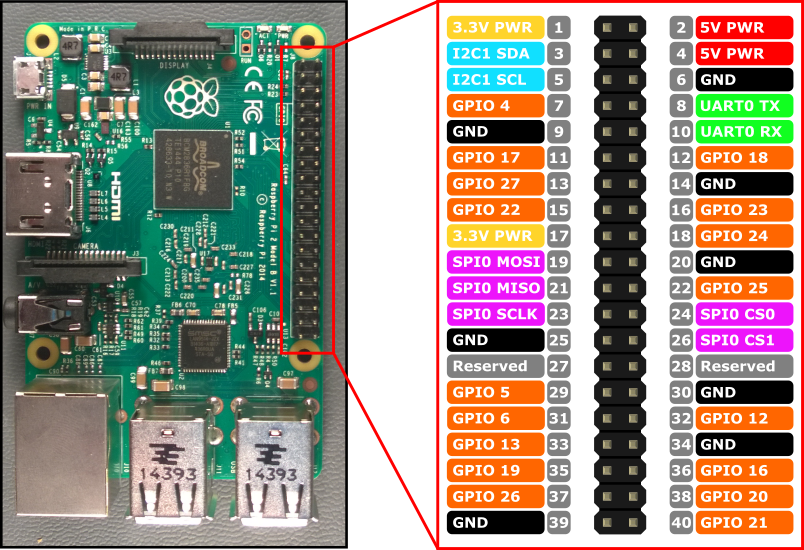
\includegraphics[width=12cm]{rpipinout}
	\caption{Rozkład pinów GPIO na płytce Raspberry Pi} 
	\label{pic:rpipinout}
\end{figure}



\subsection{Płytka pomiarowa}

Płytka pomiarowa, stanowiąca rozszerzenie do Raspberry Pi, miała umożliwiać podłączenie czujników do minikomputera oraz doprowadzenie do nich zasilania i została wykonana na potrzeby pracy dyplomowej. 
Zastosowanie przetwornika analogowo-cyfrowego pozwala na zbieranie danych z czujników analogowych. Czujniki cyfrowe podłączone przez magistralę SPI lub I$^2$C powinny być wydajnie obsługiwane przez system.

\subsection{Założenia oprogramowania}

Oprogramowanie powinno umożliwiać przeprowadzenie wydajnej akwizycji, bez utraty danych.
Niezbędne jest skorzystanie z odpowiednich bibliotek i funkcji udostępnianych przez jądro systemu Linux. Aplikacje użytkownika powinny zapisywać dane do pliku w formacie umożliwiającym późniejsze przetworzenie przez aplikację obsługującą protokół sieciowy MQTT i aplikację umożliwiającą wyświetlanie danych i ustawienie konfiguracji parametrów pomiaru uruchamianą przez użytkownika w przeglądarce internetowej. Aplikacja udostępnia interfejs pozwalający na zdalne uruchomienie programów obsługujących Oprogramowanie powinno posiadać cechy przenośności tak, aby mogło działać na innych systemach wbudowanych z systemem operacyjnym Linux.


\chapter{Projekt}
\label{ch:projekt}

\section{Płytka pomiarowa}

Płytka pomiarowa składa się z dwóch przetworników ADC podłączonych przez odpowiednie interfejsy do wejść komputera Raspberry Pi. Zasilanie układów jest doprowadzone z wyjść zasilających Raspberry Pi. W celu wytłumienia zakłóceń dodano elementy pasywne o odpowiednich wartościach. Sygnały do przetwornika z oscyloskopu doprowadzono przy pomocy kabli BNC i odpowiednich końcówek.
Na Rys. \ref{fig:schplytki} przedstawiono schemat płytki zawierającej przetwornik analogowo-cyfrowy MAX1202 oraz wyjścia cyfrowe i analogowe do podłączenia zewnętrznych czujników. Wyprowadzono także wejścia interfejsu UART w celu komunikacji z komputerem.


\begin{figure}[h]
	\centering
		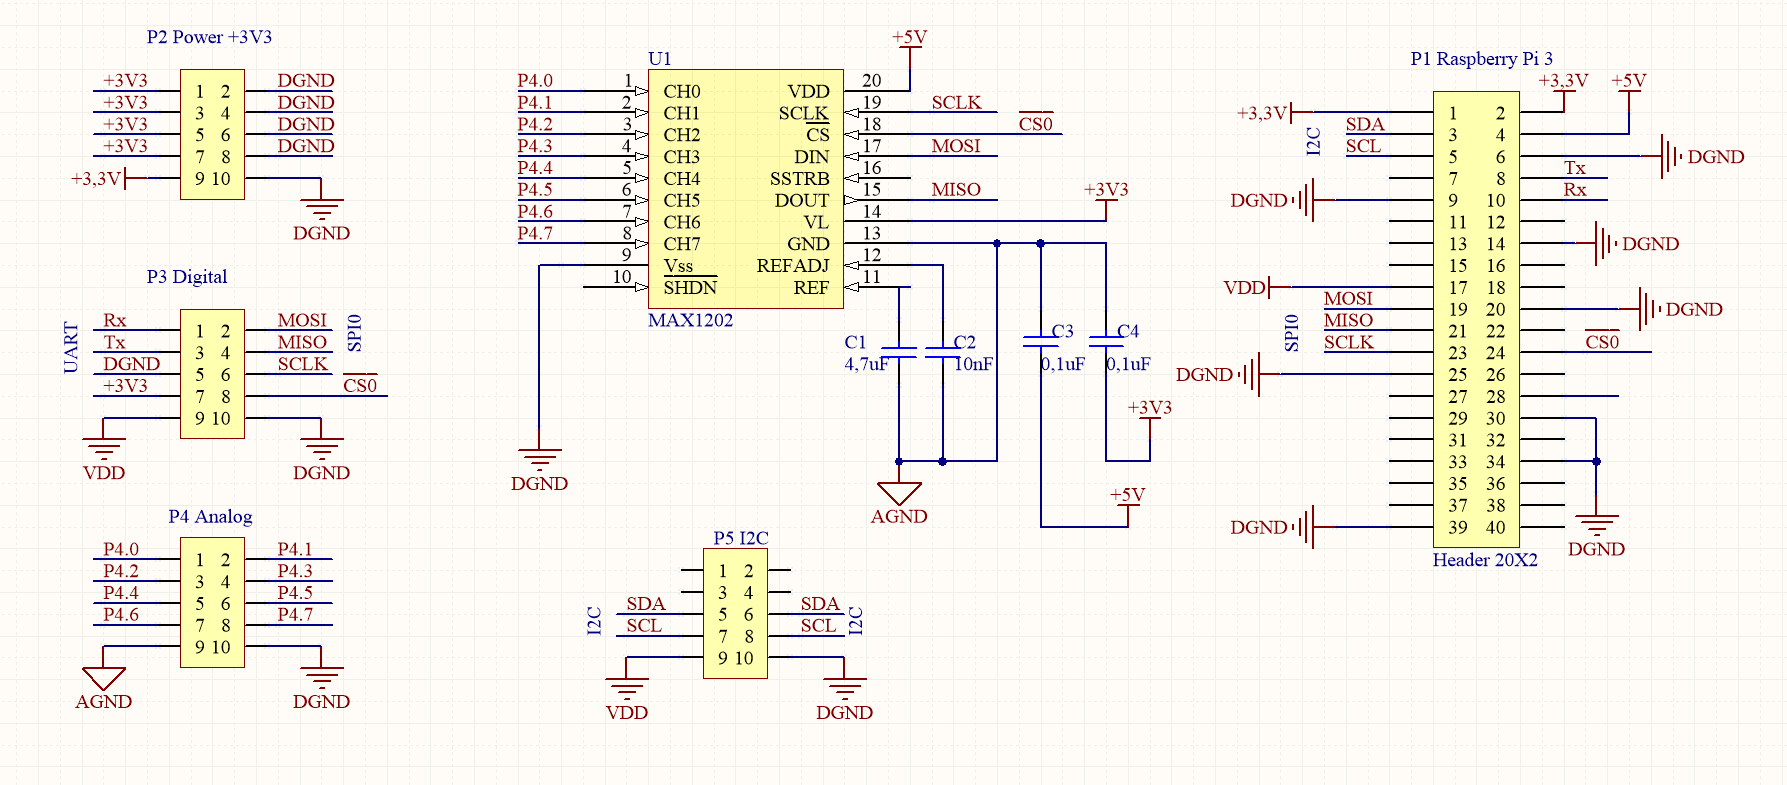
\includegraphics[width=14cm]{schplytki}
	\caption{Schemat płytki dołączanej do Raspberry Pi} 
	\label{fig:schplytki}
\end{figure}

Na Rys.\ref{fig:plytka3d} trójwymiarowy wygląd płytki wygenerowany w programie Altium PCB Designer. 

\begin{figure}[h]
	\centering
		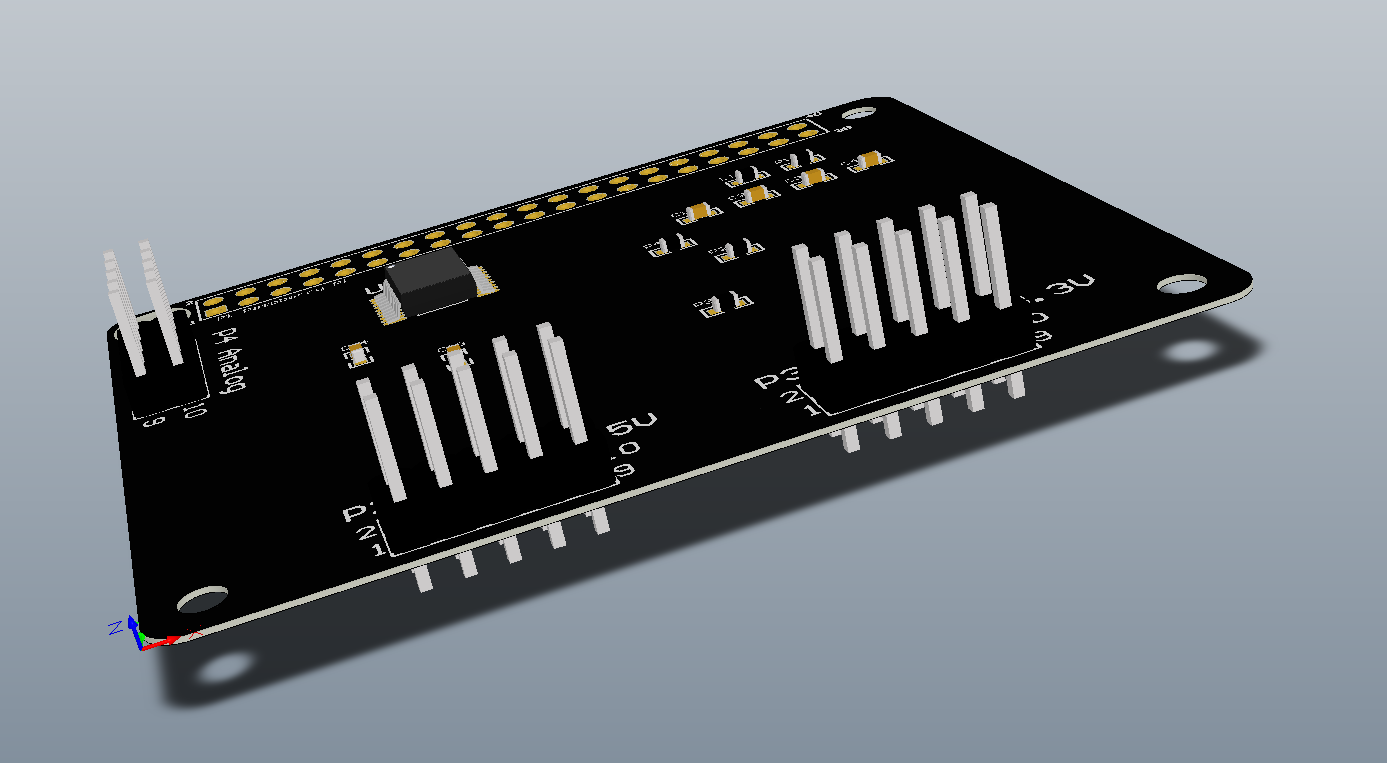
\includegraphics[width=14cm]{plytka3d}
	\caption{Trójwymiarowy wygląd projektu płytki} 
	\label{fig:plytka3d}
\end{figure}

Ze względu na ograniczenia czasowe i optymalizację projektu pod względem kosztu podjęto decyzję zmontowania układu na płytce prototypowej. Wygląd płytki bez zamontowanych elementów przedstawiono na Rys \ref{fig:rpihat}

\begin{figure}[h]
	\centering
		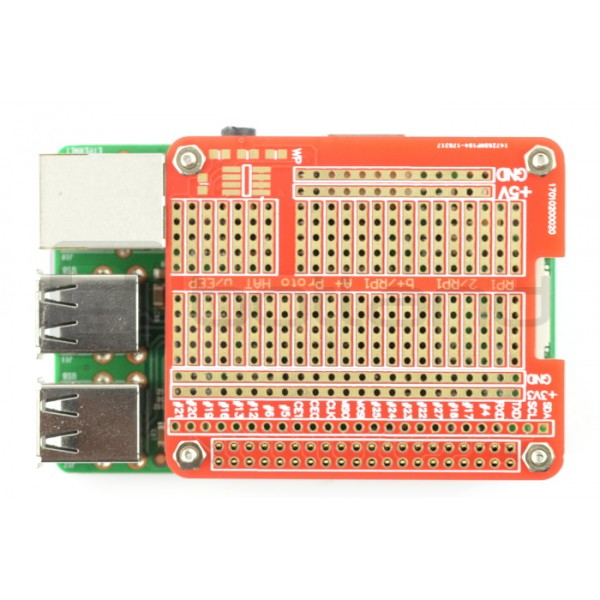
\includegraphics[width=12cm]{rpihat}
	\caption{Płytka prototypowa dołączana do Raspberry Pi 2/3} 
	\label{fig:rpihat}
\end{figure}


\section{Przetwornik analogowo-cyfrowy}

\subsection{Analiza dostępnych układów}
Przy wyborze przetwornika zwrócono uwagę na następujące parametry:
\begin{itemize}
\item cena układu, 
\item rozdzielczość, 
\item częstotliwość próbkowania,
\item interfejs komunikacji,
\item zasilanie i poziomy logiczne
\end{itemize}

\subsection{Przetwornik MAX 1202}

Jednym z wybranych układów był 12-bitowy, 8-kanałowy przetwornik MAX 1202 o próbkowaniu 133 kS/s. Komunikacja z układem odbywa się przez interfejs szeregowy SPI, a poziomy logiczne mogą być ustawione na wartość w zakresie 2,7V - 5,5V w zależności od napięcia podanego na pin VL. Do komunikacji z Raspberry Pi potrzebne są poziomy 3,3V, więc należy podać napięcie 3,3V na odpowiedni pin przetwornika ADC. Układ może być zasilany napięciem 5V.
Podłączenie przetwornika analogowo cyfrowego przez interfejs SPI do platformy Raspberry Pi przebiegało jak na Rys. \ref{fig:maxandrpi} Przetwornik zasilono korzystając z jednego z wyjść +5V dostępnych na płytce. Korzystając z zaleceń producenta zawartych w nocie katalogowej \cite{maxdatasheet} podłączono kondensatory tłumiące niekorzystne dla dokładności pomiaru zakłócenia.  


\begin{figure}[h]
	\centering
		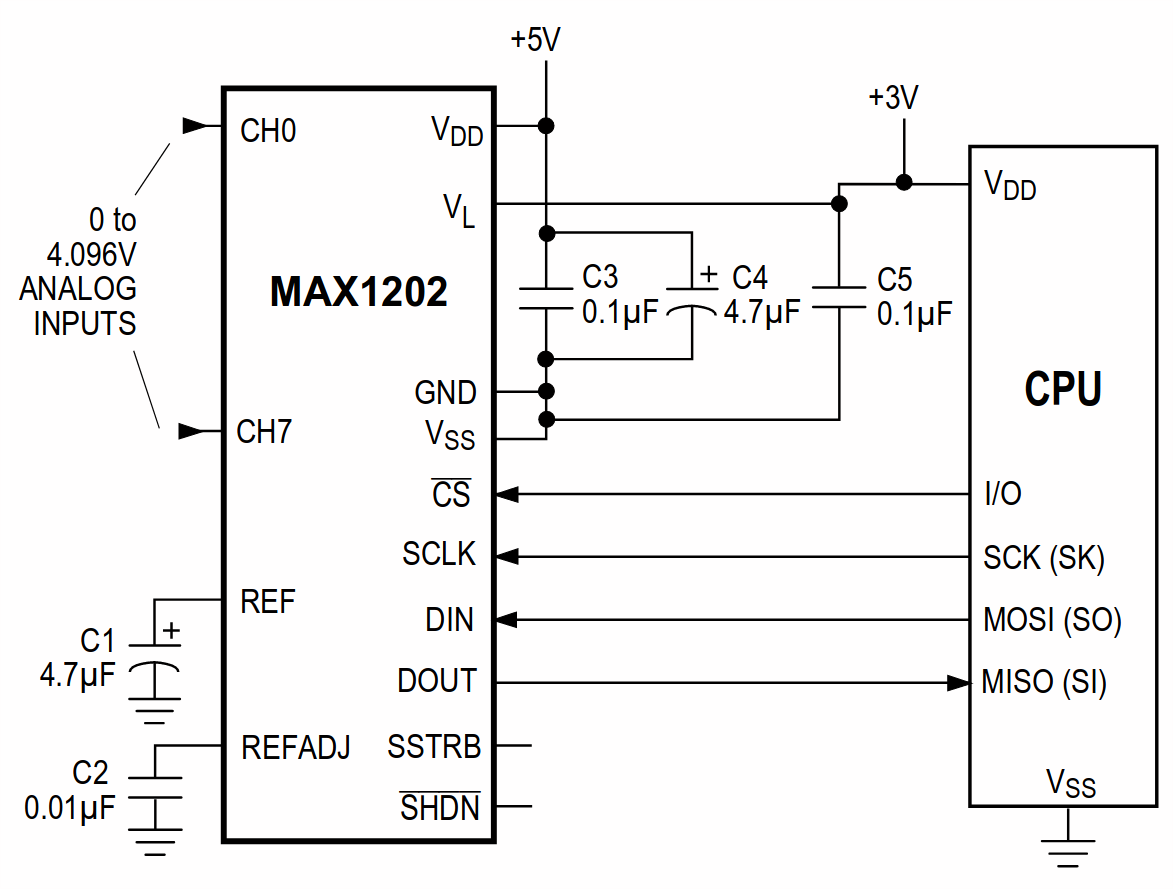
\includegraphics[width=10cm]{max1202_sch}
	\caption{Schemat podłączenia przetwornika MAX1202 do systemu} 
	\label{fig:maxandrpi}
\end{figure}

Na Rys. \ref{fig:maxczasowy} przedstawiono przebiegi czasowe napięć na poszczególnych liniach interfejsu w trakcie jednej konwersji napięcia. Jak widać transmisja jednej próbki napięcia odbywa się po przesłaniu jednego bajtu konfiguracyjnego wysłanego z układu typu Master. Przetwornik dokonuje konwersji napięcia analogowego z wybranego kanału i wysyła dwa bajty zawierające dane. Z wykresu odczytać można parametr \ang{ACQUISITION} wynoszący 1,5 $\mu$s. 


\begin{figure}[h]
	\centering
		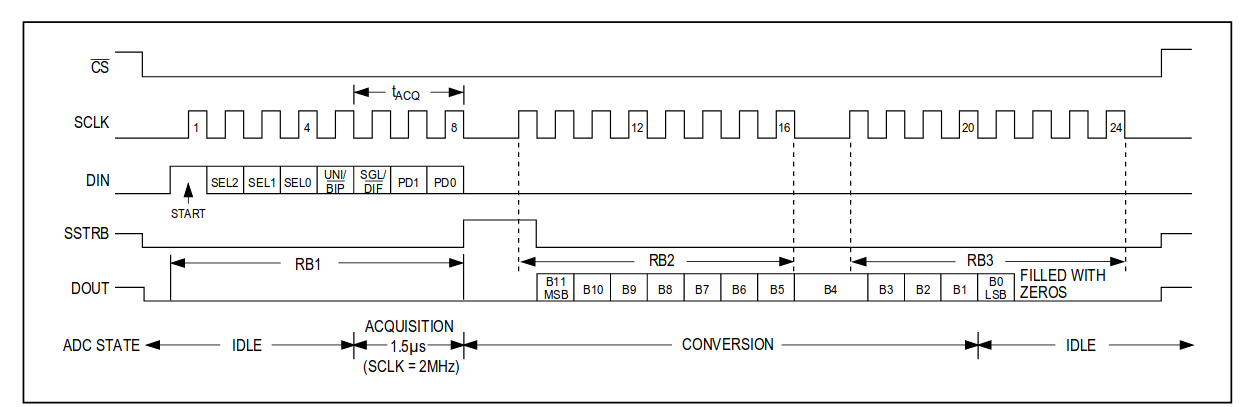
\includegraphics[width=14cm]{max1202time}
	\caption{Wykres czasowy konwersji przetwornika ADC MAX1202} 
	\label{fig:maxczasowy}
\end{figure}


\subsection{Przetwornik MCP 3424}

Drugi testowany układ to 18-bitowy 4-kanałowy przetwornik MCP 3424. Przetwornik komunikuje się z systemem za pomocą interfejsu I2C i posiada wbudowany wzmacniacz programowalny (PGA - z ang Programmable Gain Amplifier). W układzie dostępne jest również źródło napięcia referencyjnego 2.048V oraz oscylator.

\begin{figure}[h]
	\centering
		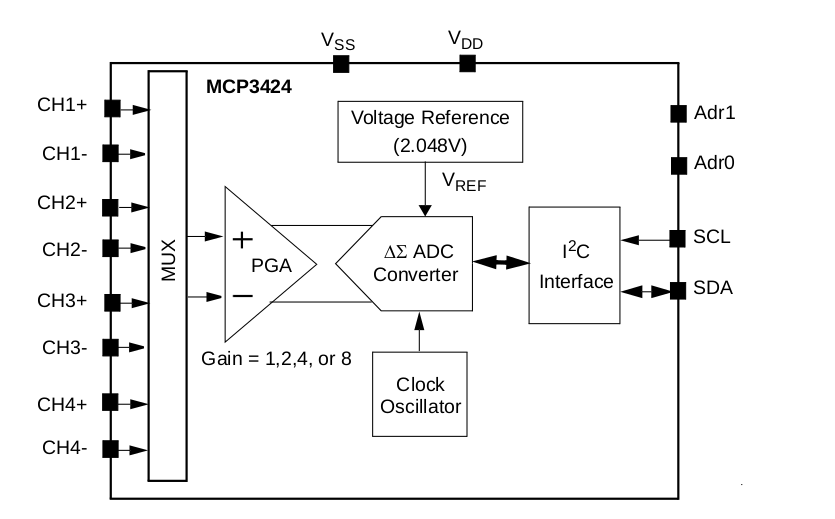
\includegraphics[width=10cm]{mcp3424_fun}
	\caption{Schemat funkcjonalny układu przetwornika MCP3424} 
	\label{fig:uxtouch}
\end{figure}


\begin{table}[t]
\label{tab3.1}
\begin{tabular}{|l|l|l|}

  \hline 
  Nazwa przetwornika & MAX1202 & MCP3424\\
  \hline
  Typ przetwornika & SAR & Sigma Delta\\
  \hline
  Ilość wejść & 8 (4 różnicowe)  & 4 różnicowe \\
  \hline 
  Interfejs komunikacji & SPI & I2C\\
  \hline
  Maksymalna częstotliwość próbkowania & 133 kS/s & 240 SPS (12bit) \\
  \hline
  Cena(w serwisie farnell.com [PLN]) & 49,63 & 16,42 \\
  \hline
  Wzmacniacz programowalny & brak & x1, x2, x4 lub x8 \\
  \hline
  
\end{tabular}
\caption{Parametry techniczne wybranych przetworników} 
\end{table}


\section{Interfejs SPI}

Interfejs szeregowy SPI (z ang. Serial Peripheral Interface)
jest powszechnie wykorzystywanym synchronicznym interfejsem do komunikacji pomiędzy systemem mikroprocesorowym, a układami peryferyjnymi. Interfejs pozwala na podłączenie tylko jednego układu typu Master komunikującego się z układami typu Slave w trybie full-duplex. Urządzenia podłączone do jednej magistrali muszą mieć jednakowe poziomy logiczne.

\newpage

Transmisja odbywa się za pomocą czterech linii:
\begin{itemize}
\item MISO (Master In Slave Out), 
\item MOSI (Master Out Slave In),
\item SCLK (Serial Clock),
\item CS (Chip Select).
\end{itemize}

Przetwornik, którego użyto jest w stanie komunikować się przy częstotliwości taktowania zegara do 2MHz. Urządzenie zostało podłączone do Raspberry Pi jako układ typu Slave. Sygnał zegara jest podawany z układu typu Master, więc w celu uniknięcia błędów transmisji należy ustawić parametr maksymalnej częstotliwości zegara w sterowniku. 


\section{Interfejs I$^2$C}

Interfejs I$^2$C (również IIC - Inter Integrated Circuit - z ang. pomiędzy układami scalonymi) to synchroniczny interfejs szeregowy zaprojektowany przez firmę Philips. Stosowany jest do komunikacji z urządzeniami nie wymagającymi dużych szybkości transmisji. Interfejs pozwala na podłączenie do magistrali wiele urządzeń typu Master oraz typu Slave. Wszystkie nadajniki posiadają wyjścia typu otwarty kolektor co powoduje, że poziomy logiczne napięć stanu wysokiego układów podłączonych do jednej magistrali mogą się różnić. Urządzenia komunikujące się za pomocą tego interfejsu mają z góry przypisany adres i są podłączone z resztą urządzeń za pomocą dwóch linii: 
\begin{itemize}
\item SDA (Serial Data Line),
\item SCL (Serial Clock Line).
\end{itemize}

Interfejs I$^2$C nie gwarantuje stałego czasu transmisji, więc korzyści wynikające z implementacji obsługi w kodzie sterownika są mniejsze. Biorąc to pod uwagę założono, że przetworniki podłączane do systemu za pomocą magistrali I$^2$C będą służyły do pomiarów z niską częstotliwością próbkowania.

\section{Porównanie dostępnych interfejsów}

Porównanie zostało wykonane pod kątem zastosowania do połączenia układów w systemie akwizycji danych. W tabeli 3.1 przedstawiono zestawienie parametrów technicznych standardów transmisji interfejsów SPI oraz I$^2$C. 


\begin{table}[!ht]
\label{tab3.2}
\begin{tabular}{|l|l|l|}
  \hline 
  Nazwa interfejsu & SPI & I$^2$C\\
  \hline
  Ilość linii sygnałowych & 3 + n(ilość urządzeń)  & 2 \\
  \hline  
  Maksymalna częstotliwość zegara & 125MHz  & 3,2MHz \\
  \hline
  Adresacja urządzeń & linia CS & 10-bitowa  \\
  \hline
  Ilość układów typu Master & 1 & może być wiele\\
  \hline
  Rodzaj transmisji & full-duplex & half-Duplex\\
  \hline
  
\end{tabular}
\caption{Parametry transmisji interfejsów SPI i I2C} 
\end{table}

\section{Pozostałe czujniki podłączane do systemu przez magistralę I$^2$C}

W celu wykonania akwizycji danych pomiarowych wykorzystano dwa moduły z czujnikami ciśnienia, wilgotności powietrza oraz temperatury. Układy są  podłączane przez magistralę I$^2$C do płytki Raspberry Pi. Moduły zawierają sensory mierzące wartości warunków atmosferycznych w postaci układów scalonych typu MEMS (z ang. Micro Electro-Mechanical System - Mikrosystemy elektromechaniczne).

\subsection{Moduł z czujnikiem ciśnienia i temperatury LPS25H}

Moduł LPS25H od firmy Pololu zawiera barometr mierzący ciśnienie atmosferyczne w zakresie: 260 mbar - 1260 mbar (26 kPa - 126 kPa). W trybie wysokiej rozdzielczości czujnik mierzy z dokładnością 0,2 mbar (0,02kPa).

\begin{figure}[h]
	\centering
		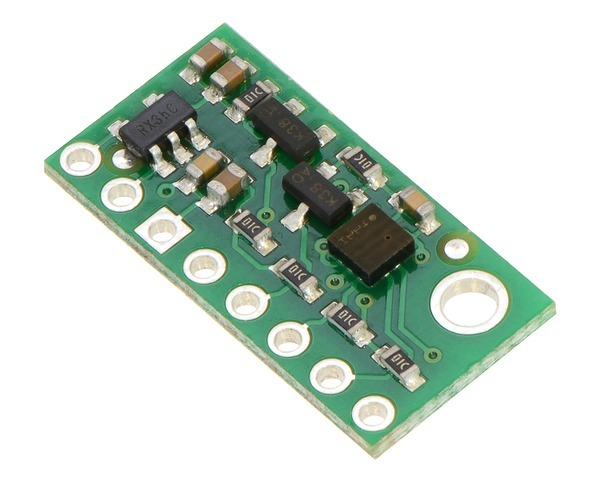
\includegraphics[width=10cm]{pololu}
	\caption{Moduł z czujnikiem ciśnienia i temperatury Pololu LPS25} 
	\label{pic:pololu}
\end{figure}

\subsection{Moduł z czujnikiem wilgotności i temperatury z układem HTS221}

Moduł HTS221 zawiera sensor wilgotności i temperatury firmy STMicroelectronics. Zakres pomiaru temperatury to 0 - 60\degree C, a wilgotności powietrza: 0 - 100\%. Układ obsługuje interfejsy I$^2$C lub SPI. Na płytce znajduje się konwerter poziomów napięć co umożliwia współpracę układu z urządzeniami o poziomach 3,3V oraz 5V i stabilizator napięcia.

\begin{figure}[t!]
	\centering
		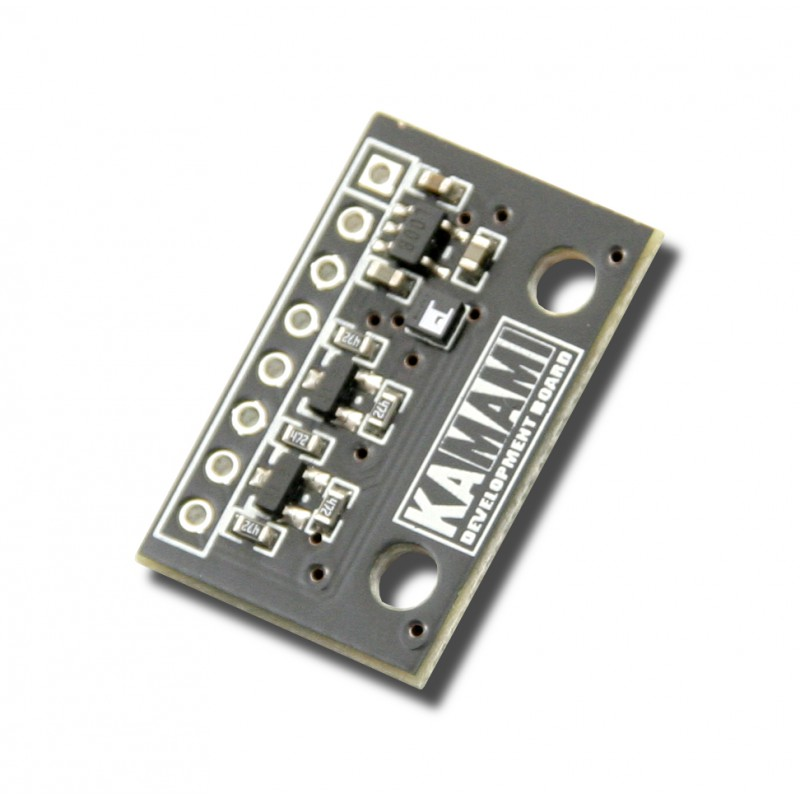
\includegraphics[width=8cm]{hts221}
	\caption{Moduł z czujnikiem wilgotności i temperatury HTS221} 
	\label{pic:hts221}
\end{figure}

Moduły miały podobny rozstaw pinów co umożliwiło podłączenie ich do wspólnej szyny.

\begin{figure}[b!]
	\centering
		\includegraphics[width=10cm]{rpiczujniki}
	\caption{Podłączenie zewnętrznych czujników do płytki} 
	\label{pic:rpiczujniki}
\end{figure}

\chapter{Oprogramowanie}
\label{ch:soft}

\section{System operacyjny}
Najczęściej używanym systemem operacyjnym na platformie Raspberry Pi jest Raspbian. Jest to
darmowa dystrybucja Linuxa oparta na Debianie, odpowiednio dostosowana do pracy z Respberry Pi. System jest udostępniony przez twórców na stronie organizacji \cite{raspfoundation} Raspberry Pi Foundation zarówno w wersji 'Raspbian with Desktop' ze środowiskiem graficznym PIXEL (z ang. Pi Improved Xwindows Environment, Lightweight), jak i w wersji bez środowiska graficznego Raspbian Lite.

Raspbian jest wielozadaniowym systemem operacyjnym, więc przydziela wszystkim programom czas procesora według algorytmu szeregowania. Z punktu widzenia aplikacji użytkownika nie wiadomo kiedy nastąpi wywłaszczenie i na jak długo. Jest to problematyczne w przypadku obsługi krytycznych czasowo zadań.
Rozwiązaniem może być zastosowanie modułu do jądra systemu operacyjnego i wykonanie krytycznych czasowo zadań w funkcji obsługi przerwania lub uruchomienie aplikacji na systemie czasu rzeczywistego (z ang. RTOS - Real Time Operating System) takim jak FreeRTOS lub ChibiOS. Systemy operacyjne czasu rzeczywistego zawierają mechanizmy ułatwiające implementacje systemu akwizycji danych. 
Podczas kompilacji jądra Linuxa istnieje możliwość dodania rozszerzeń czasu rzeczywistego, które udostępniają funkcje w przestrzeni jądra i użytkownika, ułatwiające implementację krytycznych czasowo aplikacji w systemie.

\section{Środowisko Buildroot}

Buildroot jest narzędziem umożliwiającym użytkownikowi stworzenie okrojonej na potrzeby danego zastosowania wersji systemu wbudowanego Linux. Środowisko to składa się z zestawu plików Makefile i kconfig, które upraszczają przygotowanie cross-kompilacji za pomocą zestawu narzędzi \ang{toolchain} dla danej architektury. Producent dostarcza również domyślne konfiguracje do kilku popularnych platform m.in. Cubieboard i Raspberry Pi, co skraca czas rozpoczęcia projektu systemu. W pobranym ze strony producenta pliku w katalogu \ang{board} (Rys. 4.1) znajduje się katalog raspberrypi zawierający domyślną konfigurację dla platformy Raspberry Pi 3.
\begin{figure}[h]
	\centering
		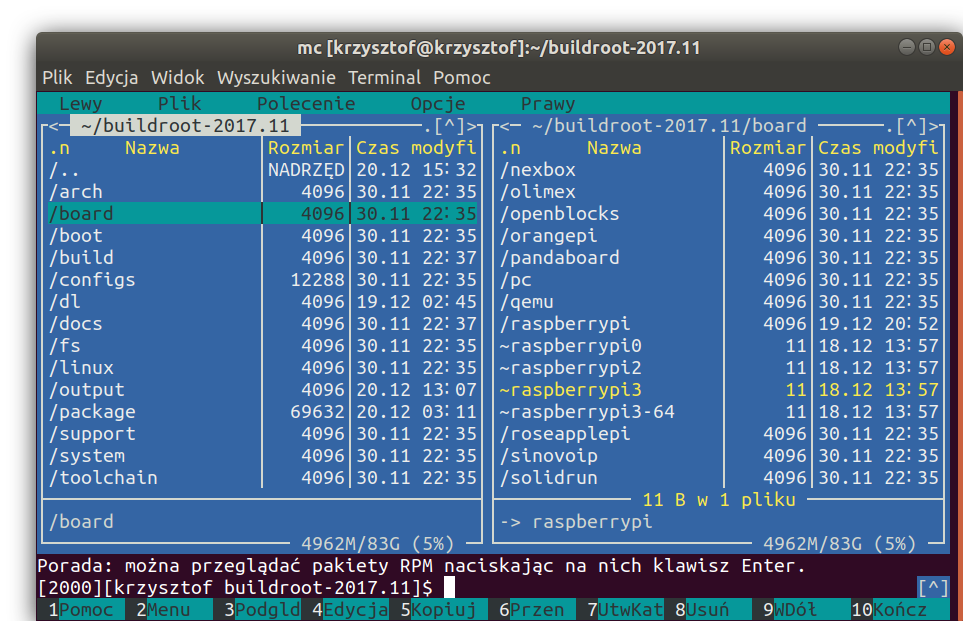
\includegraphics[width=10cm]{buildroot_katalogi}
	\caption{Katalog board z plikami konfiguracyjnymi} 
	\label{fig:uxtouch}
\end{figure}

Buildroot pozwala ustawić opcję dwóch rozszerzeń czasu rzeczywistego XENOMAI i RTAI. Są to rozszerzenia wykorzystywane w systemach wbudowanych do wspierania aplikacji czasu rzeczywistego.
RTAI (z ang. real time application interface - interfejs dla aplikacji czasu rzeczywistego) jest dostępny w środowisku Buildroot dla 64-bitowej architektury procesora Raspberry Pi 3. Moduły RTAI umożliwiają ustawienie priorytetu wywłaszczalności każdej aplikacji w systemie, co pozwala na zapewnienie poprawności działania krytycznych czasowo zadań.


\subsection{Interfejs środowiska}
Buildroot tworzy system plików, kompiluje jądro systemu Linux i generuje \ang{boot loader}. Konfiguracja kompilacji systemu jest ustawiana w menu głównym środowiska Buildroot (Rys. 4.2.) za pomocą interfejsu wywoływanego komendą \ang{make menuconfig}.

\begin{figure}[h]
	\centering
		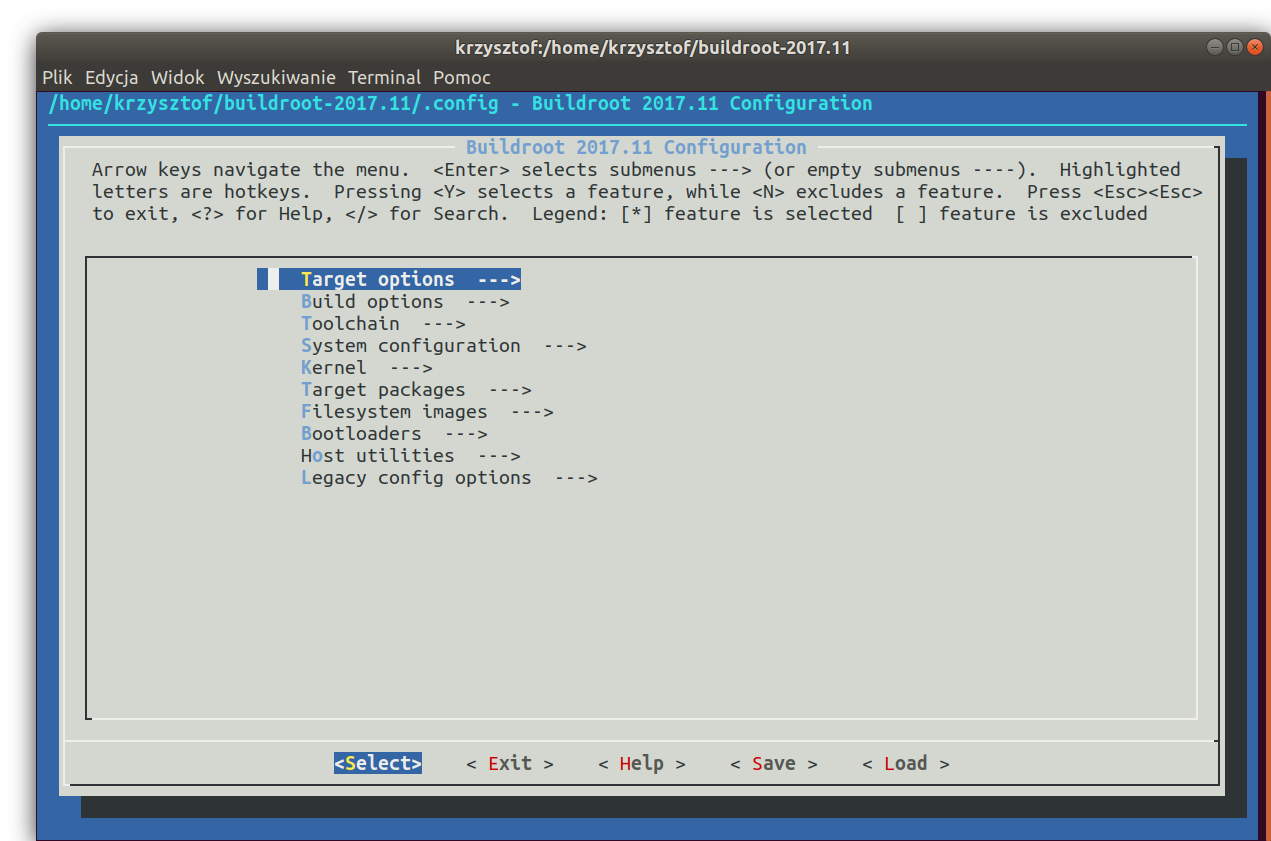
\includegraphics[width=10cm]{buildroot_menu}
	\caption{Widok głównego menu środowiska} 
	\label{fig:uxtouch}
\end{figure}

\subsection{Toolchain}

Toolchain jest zestawem narzędzi programistycznych, pozwalających na wykonanie cross-kompilacji programu na maszynie o innej architekturze. Składa się z kompilatora, linkera oraz bibliotek danego języka programowania. W środowisku Buildroot użytkownik ma możliwosć wybrania, czy Toolchain ma być stworzony przez środowisko zgodnie z opcjami dotyczącymi architektury sprzętu docelowego. Alternatywą jest podanie zewnętrznego zestawu narzędzi \ang{Toolchain} i dołączenie do projektu.

\subsection{Dodawanie modułów jądra}

Dodawanie skompilowanych modułów jądra odbywa się za pomocą komendy \ang{modprobe}. Kod modułu wraz z plikami konfiguracyjnymi należy dodać podczas konfiguracji środowiska Buildroot. Na etapie dokonywania zmian w kodzie sterownika, Buildroot umożliwia cross-kompilację wybranego pakietu. Skompilowany moduł wysyłano za pomocą połączenia ssh.


\section{Komunikacja z Raspberry Pi}

Na etapie rozwoju oprogramowania, debugowania oraz testów potrzebna była komunikacja pomiędzy komputerem PC, a płytką Raspberry Pi. Platforma posiada kilka różnych możliwości komunikacji, jednak najbardziej niezawodnym i dającym pełną informację o stanie systemu był port UART. Aby móc obsłużyć konwerter USB-UART i komunikować się z Raspberry Pi na komputerze PC posłużono się programem minicom.

Komunikacja przez port Ethernet, bądź WiFi za pomocą klienta SSH (a ang. Secure Shell) pozwalała na komunikację z większą przepustowością, co było istotne podczas testów systemu pod kątem akwizycji danych. 

\section{Sterowniki urządzeń}
Do obsługi urządzeń dołączanych do systemu przy pomocy magistral SPI i I2C potrzebne są odpowiednie sterowniki urządzeń. Można skorzystać z gotowych modułów udostępniających aplikacjom użytkownika dostęp do pamięci urządzeń takich jak np. \ang{spidev}\cite{spidev} i \ang{i2c-dev}\cite{i2cdev}. W celu zapewnienia wydajnej pracy programom o ścisłym reżimie czasowym w projekcie zastosowano moduł do jądra systemu operacyjnego umożliwiający obsługę przetwornika analogowo-cyfrowego.

\subsection{Sterownik przetwornika analogowo-cyfrowego}

Projekt zakładał napisanie kodu sterownika urządzenia umożliwiającego dostęp aplikacji do magistrali SPI w celu odebrania pomiaru napięcia analogowego z jednego z ośmiu kanałów przetwornika analogowo-cyfrowego MAX1202. Użytkownik powinien mieć możliwość ustawienia okresu próbkowania przetwornika
oraz wyzwolenia i przerwania pomiaru z poziomu aplikacji. 

Komunikacja sterownika z aplikacją jest zapewniona poprzez urządzenie znakowe kw\_adc.
Do wysyłania komend do urządzenia zastosowano funkcję ioctl(). Przed pomiarem użytkownik ustawia za pomocą ioctl z komendą ADC\_SET czas pomiędzy przerwaniami (pole adc\_sampling\_period w strukturze dev) co powoduje ustawienie okresu próbkowania przetwornika. 
W jednym transferze wysyłany jest 1 bajt komendy (pomiar z CH1 to 0x9f) i jednocześnie odbierane są 2 bajty danych pomiarowych. 

Aby zaimplementować funkcjonalność zmiany częstotliwości próbkowania z poziomu aplikacji. 
użyto struktury hr\_timer. Po skończeniu odliczania przez licznik uruchamiana jest funkcja obsługi przerwania, następuje przygotowanie odpowiednich struktur do transferu bajtów poprzez magistralę SPI. Ustawiane są parametry transmisji Pomiar jest zlecany przez funkcję spi\_async asynchronicznie, więc proces nie jest blokowany. Gdy transfer jest zakończony uruchamiana jest funkcja complete(), gdzie dane pomiarowe są wpisywane do bufora cyklicznego. Z poziomu użytkownika dane są dostępne dzięki funkcji poll(), w której proces odczytu jest usypiany jeśli w buforze nie ma wystarczającej ilości danych do czytania. Po wpisaniu danych do bufora proces oczekujący na dane jest budzony w funkcji complete().


Istotnym podczas pisania sterownika był fakt, że dane są odbierane w funkcji obsługi przerwania. Determinowało to użycie funkcji asynchronicznej, bo funkcja spi\_sync\_transfer może być usypiana, więc nie możemy użyć jej w kontekście obsługi przerwania.
Dokonując niewielkich zmian w konfiguracji zawartej w kodzie sterownika możliwe jest obsłużenie innych układów posiadających interfejs SPI. Zweryfikowaniu i ewentualnej zmianie powinny być poddane pola struktury \ang{spi\_transfer} opisującej parametry transferu spi, które są opisane w dokumentacji jądra systemu operacyjnego Linux.\cite{spiKernel}.

\subsection{Protokół synchronizacji czasu}

Aby otrzymać dokładną informację o czasie pobrania próbki z przetwornika lub czujnika potrzebna jest synchronizacja czasu pomiędzy urządzeniami, którą można zapewnić dzięki protokołowi synchronizacji czasu takim jak na przykład NTP (z ang. Network Time Protocol).
Domyślnie w systemie Raspbian Jessie działa usługa \ang{systemd-timesyncd}, która działa na podstawie protokołu SNTP (z ang. Simple NTP) i jest dużo mniej rozbudowana. W przeciwieństwie do NTP to tylko klient, który pobiera i aktualizuje czas w systemie. W przypadku gdy chcemy skorzystać z serwera NTP, najlepiej jest tę usługę wyłączyć\cite{ntp}.

\subsection{Znacznik czasu}

System akwizycji danych wraz z zapisaną wartością próbki zapisuje czas zebrania próbki. Wykorzystano czasu systemowy, który został wcześniej zsynchronizowany z serwerem NTP.
Początkowo w pierwszym podejściu do problemu zastosowano rozwiązanie w przestrzeni użytkownika, przy użyciu funkcji \ang{getMicrotime()}. Funkcja ta pozwala na zapisanie znacznika czasu w [$\mu$s] z racji na to, że jest wywoływana z programu w przestrzeni użytkownika, nie daje dużej dokładności. Nie da się jednoznacznie stwierdzić ile czasu minie pomiędzy zapisaniem wartości znacznika czasu i zebraniem próbki, ponieważ proces może być wywłaszczany.

Większą dokładność osiągnięto stosując licznik \ang{hrtimer} w kodzie modułu jądra, który pozwala na odmierzanie czasu w nanosekundach. Na zwiększoną dokładność tego rozwiązania ma wpływ fakt, iż znacznik czasu jest zapisywany w przestrzeni jądra i dopiero później przekazywany do aplikacji użytkownika.

Dokładna wartość znacznika czasu jest przechowywana w strukturze \ang{timespec}. Pobrano tą wartość dzięki funkcji getnstimeofday() zwracającej czas w nanosekundach i zapisano w zmiennej 64-bitowej. Znacznik czasu przekazywano do sterownika wraz z wartością próbki za pomocą bufora kołowego.


. Tak zebrane dane mogą być wykorzystane w aplikacji z przestrzeni użytkownika na obliczenie znacznika czasu każdej próbki. To rozwiązanie pozwala osiągnąć większą dokładność i stałość częstotliwości próbkowania.


\section{Drzewo urządzeń}
W celu uruchomienia swojego modułu do jądra napisano nakładkę na drzewo urządzeń i skompilowaną dodano do odpowiedniego katalogu /boot/overlays, a następnie dopisano w pliku /boot/config.txt nazwę nakładki. Podane w nakładce parametry transmisji danych między urządzeniem podłączonym do magistrali, a płytką Raspberry Pi są ustalane przy załadowaniu modułu. 


\section{Aplikacje w przestrzeni użytkownika}

Programy użytkownika umożliwiają wyświetlenie danych zebranych przez niższą warstwę systemu. Wyniki pomiarów są zapisywane w plikach tekstowych i udostępniane sieciowo.

\subsection{Aplikacja wykorzystująca moduł \ang{spidev}}

W celu porównania wydajności i parametrów akwizycji danych różnych rozwiązań programowych napisano program wykorzystujący moduł \ang{spidev}. Moduł ten pozwala na odczyt danych doprowadzonych do magistrali SPI z poziomu aplikacji użytkownika. W rozdziale 5 przedstawiono wyniki testów i porównanie zmienności częstotliwości próbkowania. Aplikacja daje możliwość odczytu jednorazowego lub ciągłego z zadanym opóźnieniem. Opóźnienie jest ustalane za pomocą parametru \ang{delay\_usecs}, będącego polem struktury \ang{spi\_ioc\_transfer}. Komunikacja ze sterownikiem \ang{spidev} jest zapewniona za pomocą funkcji \ang{ioctl()} z komendą \ang{SPI\_IOC\_MESSAGE}. Komenda jest wywoływana w pętli głównej programu, a odebrane dane z przetwornika są zapisywane do bufora. Następnie pomiar jest zapisywany do pliku wraz ze znacznikiem czasu.

\subsection{Programy publikujące i subskrybujące dane przy pomocy protokołu MQTT}

Programy implementujące klienta i brokera MQTT napisano w języku Python w wersji 2 wykorzystując pakiet paho.mqtt.client, który udostępnia funkcje umożliwiające w łatwy sposób implementację aplikacji. 
Aplikacja publikująca publish.py wykonywana jest na Raspberry Pi i zawiera kod, który powoduje wysyłanie w pętli kolejno zebranych próbek. Publikacja zostaje nazwana tematem 
\ang{client.publish("test\_mqtt", file\_content[l]);)}.
W aplikacji klienta subscribe.py zawarty temat subskrybcji, który musi być zgodny z tematem zawartym w aplikacji publikującej dane\cite{paho.mqtt}
client.subscribe("test\_mqtt")

Program odpowiadający za odebranie danych zawiera informację na temat połączenia sieciowego: adres IP oraz numer portu.

\subsection{Aplikacja internetowa}

Aplikacja została napisana w języku php i html. Użytkownik jest wstanie uruchomić proces oraz go wyłączyć, korzystając z identyfikatora procesu zwracanego przez funkcję  \ang{shell\_exec}. Identyfikator uruchomionego procesu zapisywany jest w pliku pid.txt. Dane zebrane przez czujniki zapisywane są w pliku tekstowym w katalogu, z którego była wywołana aplikacja. W przypadku wywołania z aplikacji internetowej jest to katalog \ang{/var/www/html}. Parametry akwizycji danych mogę być ustawiane z poziomu aplikacji internetowej i zapisane do pliku konfiguracyjnego. Informacja o parametrach pomiarów jest wczytywana z pliku konfiguracyjnego przez program obsługujący dany czujnik. Po odebraniu próbki użytkownik jest w stanie podejrzeć aktualną wartość odczytaną z sensora uruchamiając aplikacją obsługującą protokół MQTT. 


\chapter{Testy}
\label{ch:testy}

Ostatnim etapem projektu było przeprowadzenie testów, pozwalających na sprawdzenie działania wszystkich elementów systemu akwizycji danych. Przeprowadzono testy sprzętu i oprogramowania, sprawdzana była poprawność i niezawodność działania całego systemu z dołączanymi zewnętrznymi czujnikami.

 
\section{Przebieg testów}
Przeprowadzono szereg testów funkcjonalnych w celu sprawdzenia czy system spełnia założenia projektowe zawarte we wstępie pracy. 


\begin{itemize}
\item analiza częstotliwościowa z wykorzystaniem algorytmu FFT (z ang. Fast Fourier Transform - szybkiej transformaty Fouriera) sygnału sinusoidalnego z zastosowaniem odpowiedniego okna czasowego
\item sprawdzenie dokładności pomiarów przy użyciu laboratoryjnych przyrządów pomiarowych 
\item test niezawodności działania przy dużym obciążeniu aplikacji
\item sprawdzenie poprawności danych z uwzględnieniem korelacji czasowej
\item test funkcjonalny komunikacji sieciowej
\end{itemize}

\section{Użyte narzędzia}
Sprawdzenie parametrów pomiaru napięcia przetwornika analogowo-cyfrowego przeprowadzono z użyciem oscyloskopu cyfrowego z funkcją generowania przebiegów sygnałów. Fakt, iż oscyloskop był cyfrowy ułatwił analizę różnic w sygnale wyjściowym z generatora i sygnałem spróbkowanym. Pomiary na oscyloskopie przeprowadzane były z użyciem sondy oscyloskopowej. Na Rys. \ref{pic:stanowisko} przedstawiono stanowisko pomiarowe systemu akwizycji danych.

\begin{figure}[h]
	\centering
		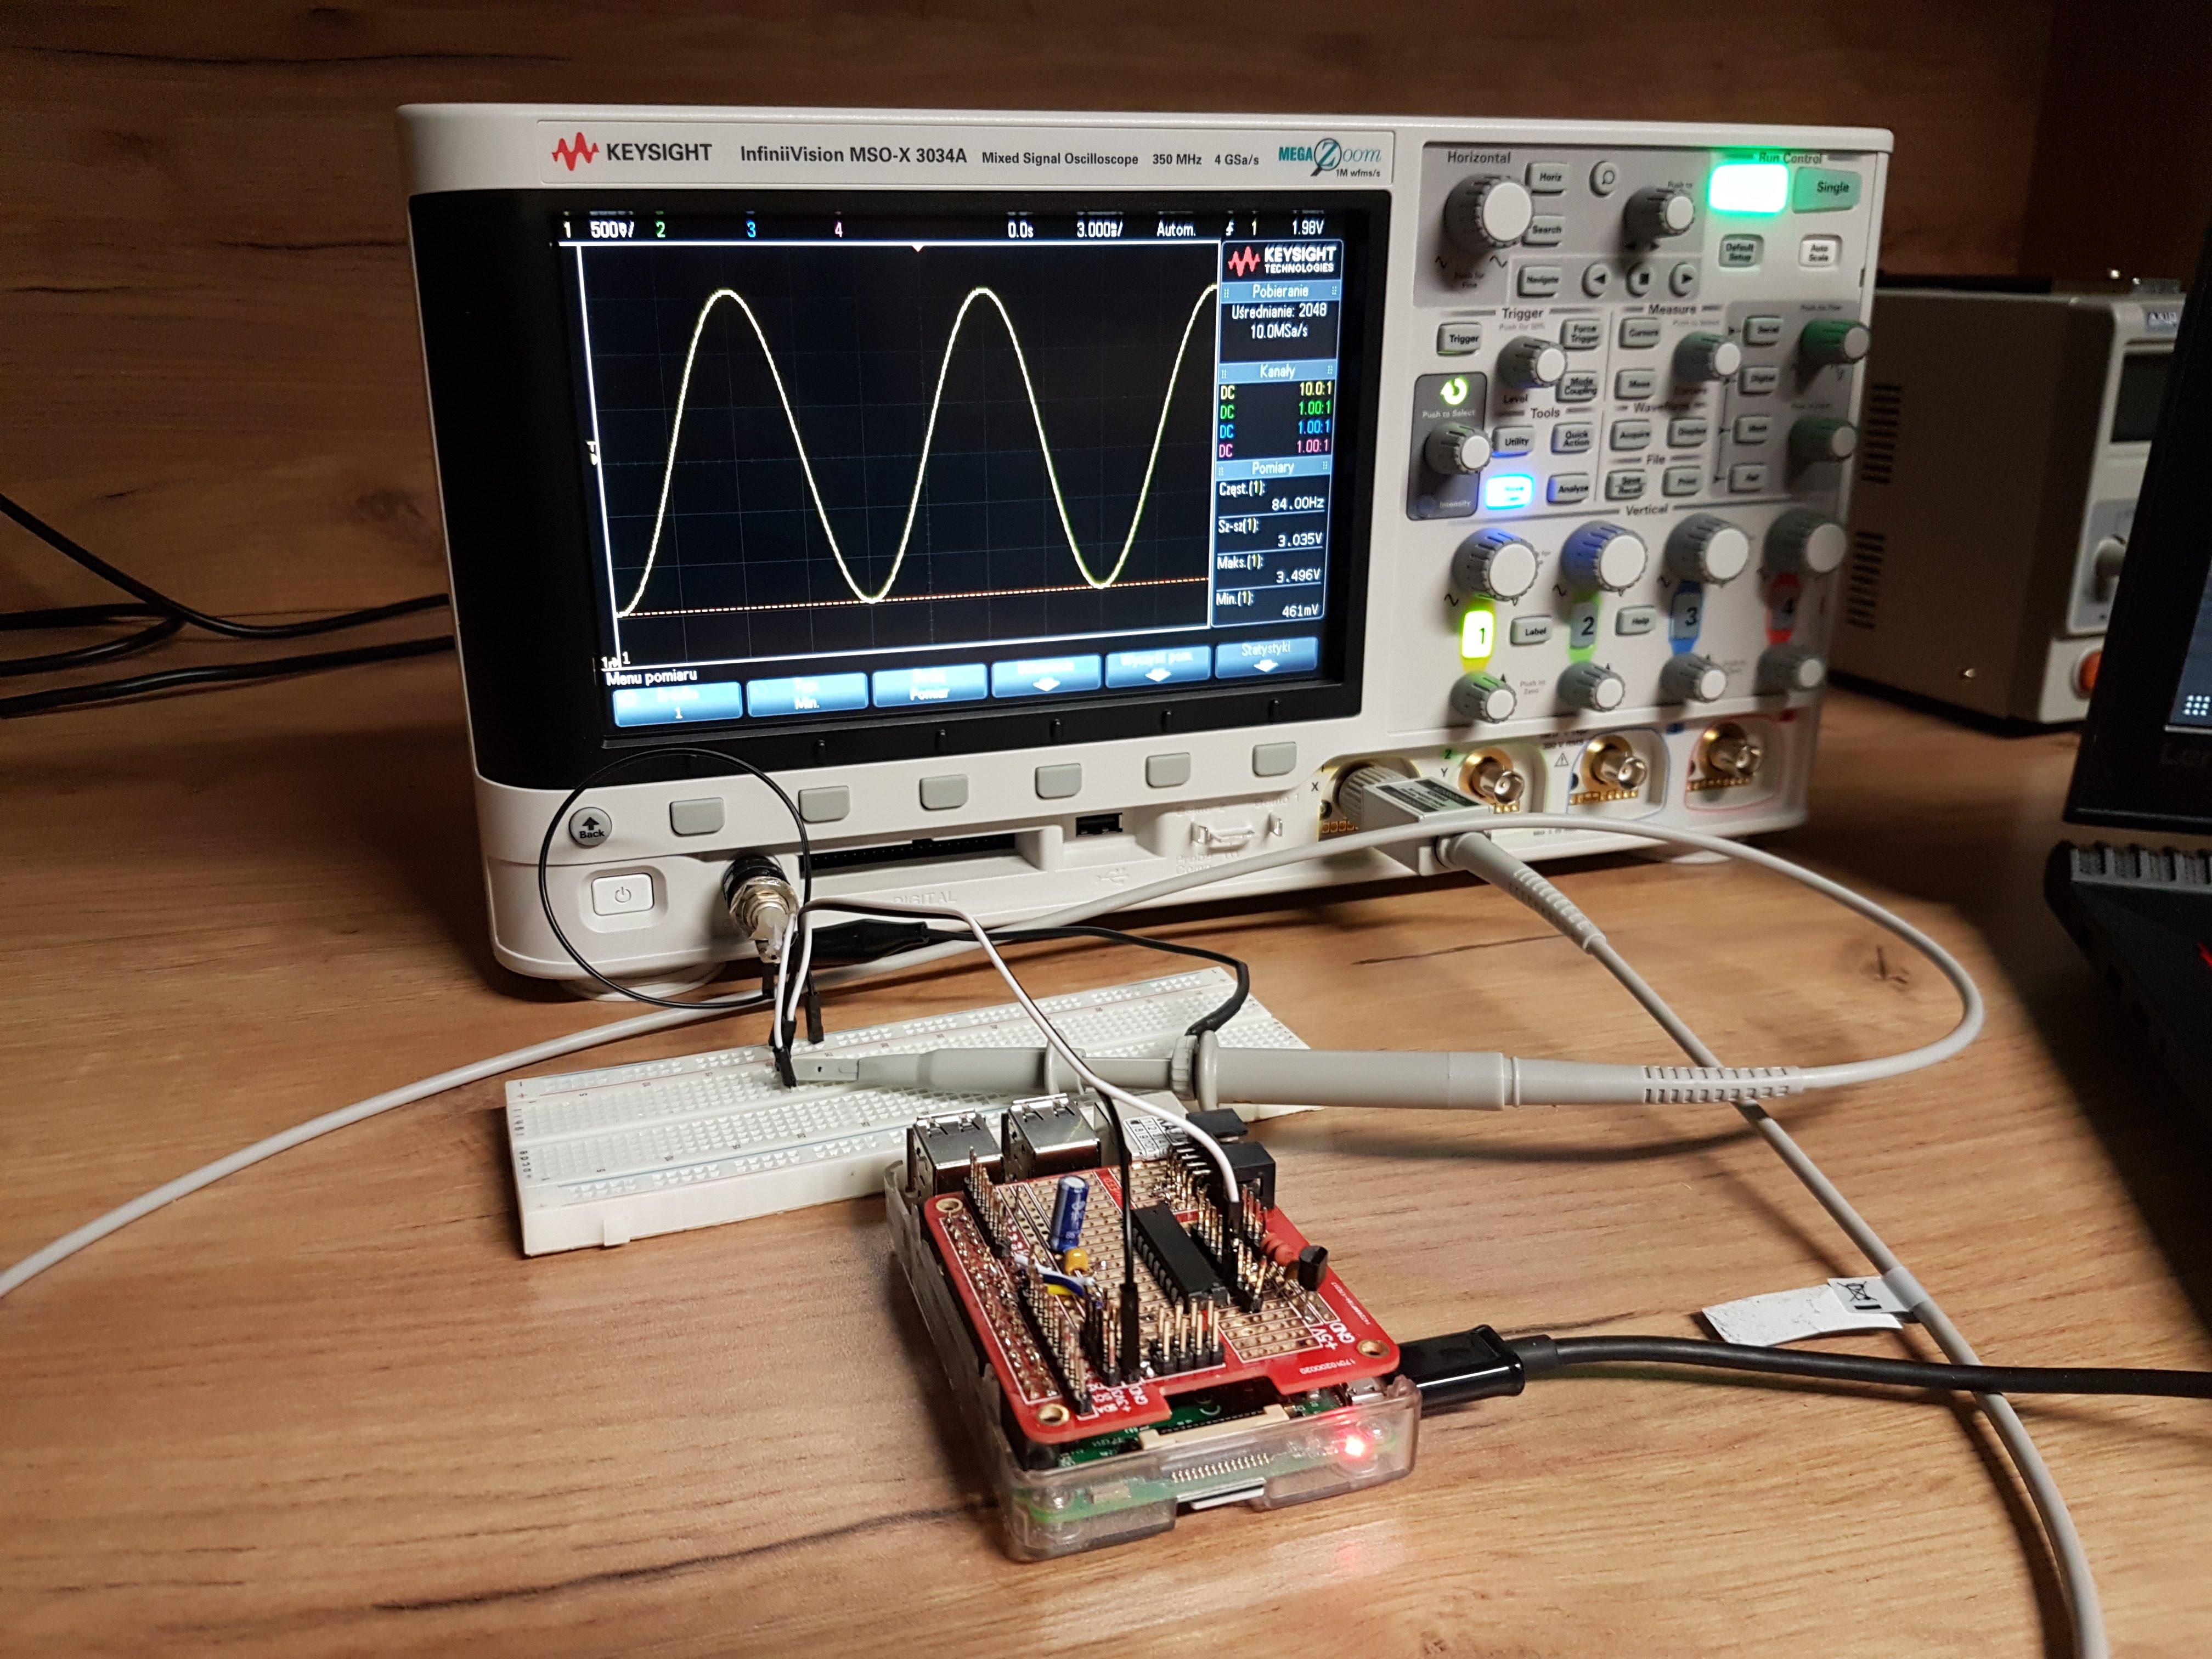
\includegraphics[width=13cm]{stanowisko}
	\caption{Stanowisko pomiarowe do pomiaru napięcia sinusoidalnego przetwornikiem analogowo-cyfrowym} 
	\label{pic:stanowisko}
\end{figure}


\section{Testy funkcjonalne}


\subsection{Test interfejsu sieciowego}

Wykonano test działania interfejsów sieciowych systemu użytkownika pod kątem spójności danych wysyłanych z systemu do użytkownika podłączonego przez sieć TCP/IP. Połączenie użytkownika korzystającego z przeglądarki w komputerze osobistym z systemem akwizycji danych było zestawione przy wykorzystaniu routera Wi-Fi.
 

\subsection{Testy niezawodności systemu}

Po ustawieniu odpowiedniej konfiguracji przeprowadzono testy niezawodności działania układu \ang{watchdog}, wywołując aplikacje powodujące zawieszenie systemu z załadowanym modułem. Oprócz konsoli \ang{ssh} podłączono komputer przez konwerter USB-UART w celu upewnienia się, że system jest uruchamiany ponownie.
Testy zakończono sukcesem, moduł sterujący układem \ang{watchdog} działał poprawnie i wywoływał ponowne uruchomienie systemu przy każdym zawieszeniu. 


\section{Wyniki pomiarów}


\subsection{Charakterystyki napięcia spróbkowanego przetwornikiem ADC MAX1202}

\subsubsection{Pomiar napięcia sinusoidalnego}

Pomiar napięcia sinusoidalnego i jego analiza częstotliwościowa, umożliwia sprawdzenie poziomu nierównomierności okresu próbkowania. 
Z oscyloskopu z funkcją generatora sygnałów wygenerowano przebieg sinusoidalny o częstotliwości 100Hz, amplitudzie 3Vp-p i składowej stałej 2V. Okres próbkowania przetwornika ustawiono w aplikacji testowej na 200us co przekłada się na częstotliwość próbkowania 5kHz. 
Spróbkowany sygnał został poddany analizie za pomocą algorytmu FFT przy użyciu skryptu pythona z pakietami \ang{numpy} i  \ang{matplotlib} .
Poniżej na Rys. \ref{fig:sin_max1202_100Hz_adc} przedstawiono fragment wykreślonego przebiegu czasowego sygnału sinusoidalnego. Linią przerywaną zaznaczono wartość średnią sygnału.

\begin{figure}[H]
	%\centering
		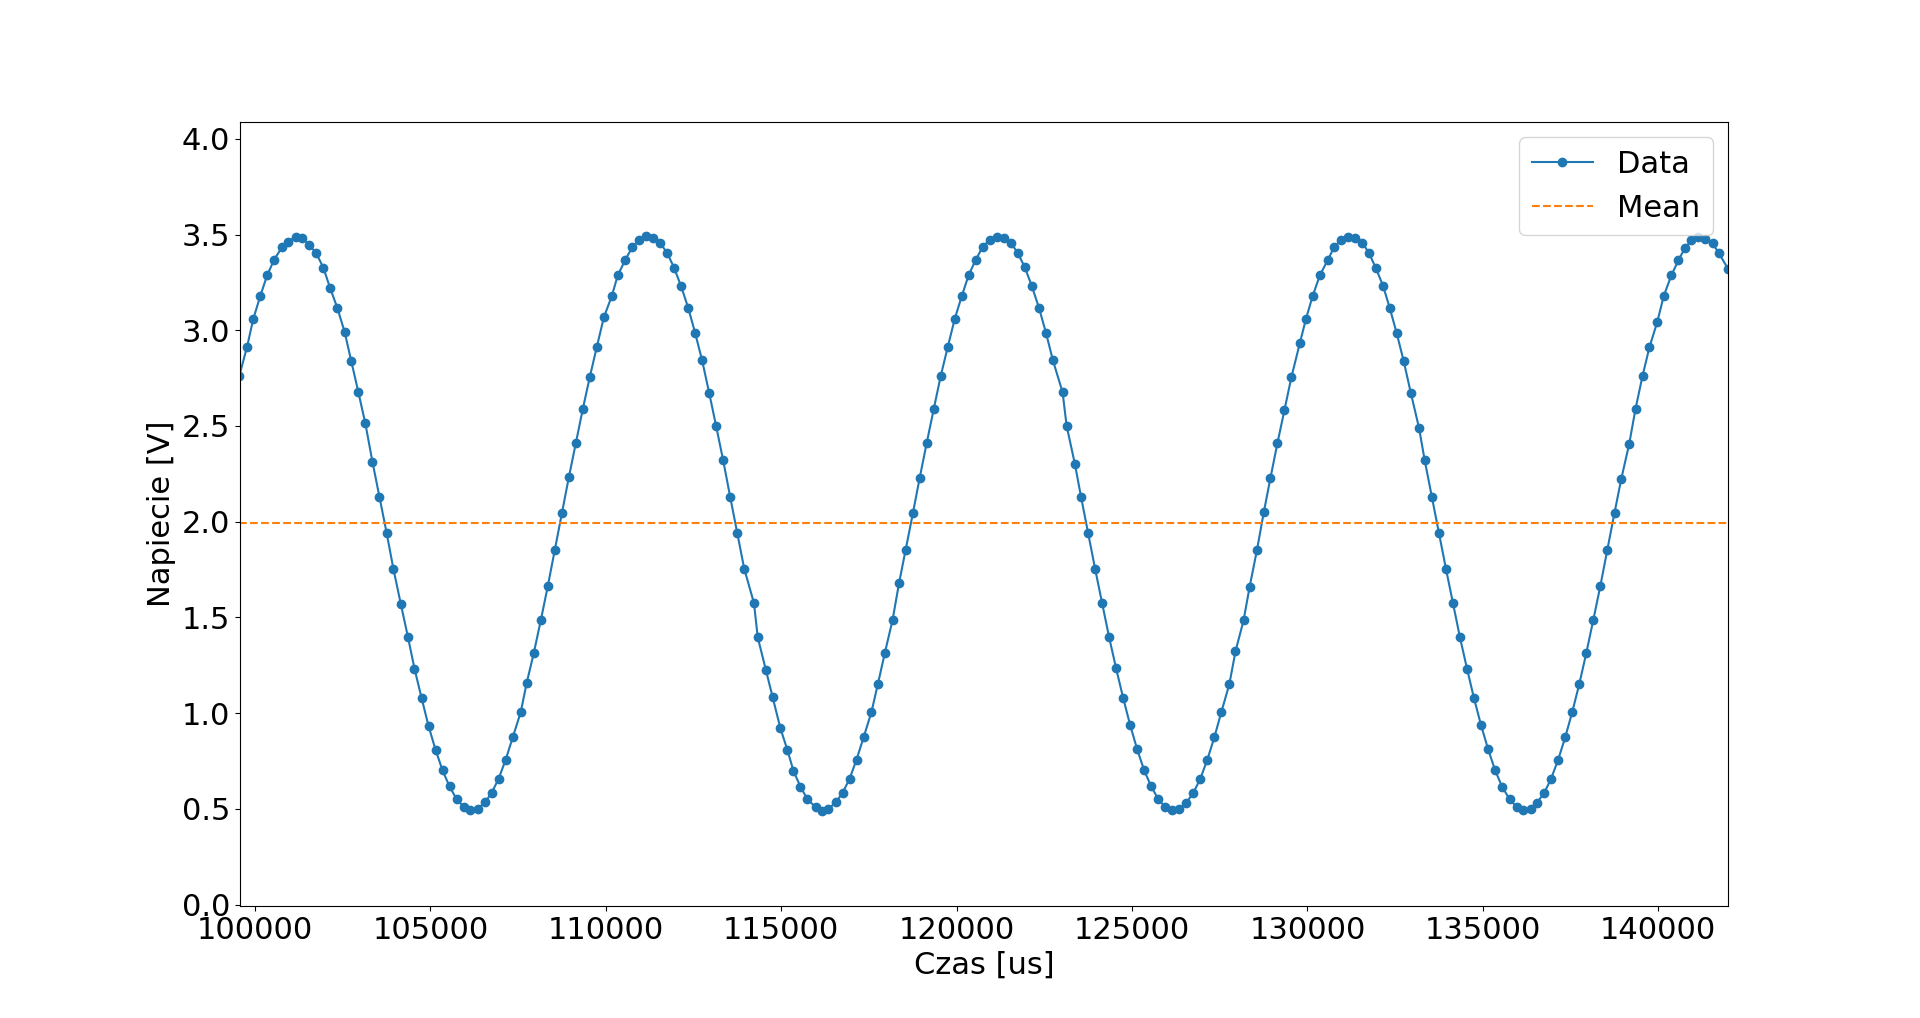
\includegraphics[width=14cm]{sin_max1202_100Hz_adc}
	\caption{Przebieg napięcia spróbkowanego przetwornika ADC MAX1202} 
	\label{fig:sin_max1202_100Hz_adc}
\end{figure}

Dla porównania sygnał z generatora zmierzono oscyloskopem przy użyciu sondy oscyloskopowej. Zrzut z ekranu oscyloskopu poniżej na Rys. \ref{fig:sin_max1202_100Hz_osc} 

\begin{figure}[H]
	\centering
		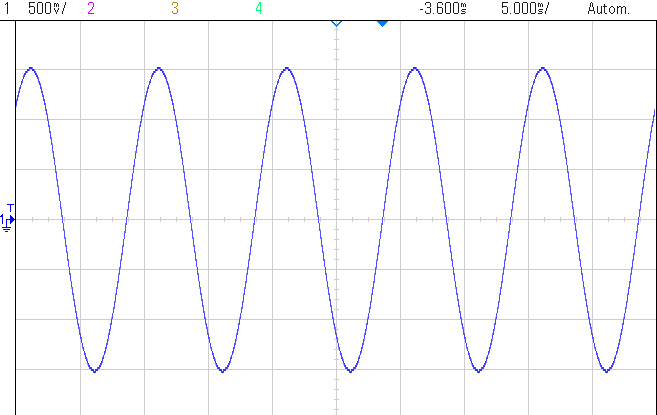
\includegraphics[width=12cm]{sin_max1202_100Hz_osc.png}
	\caption{Przebieg napięcia sinusoidalnego z oscyloskopu} 
	\label{fig:sin_max1202_100Hz_osc}
\end{figure}

Poniżej na Rys. \ref{fig:zmiennosc_probkowania_max1202} przedstawiono charakterystykę zmienności okresu próbkowania. Widać na niej jak zmienia się okres próbkowania w trakcie działania programu.

\begin{figure}[h]
	\centering
		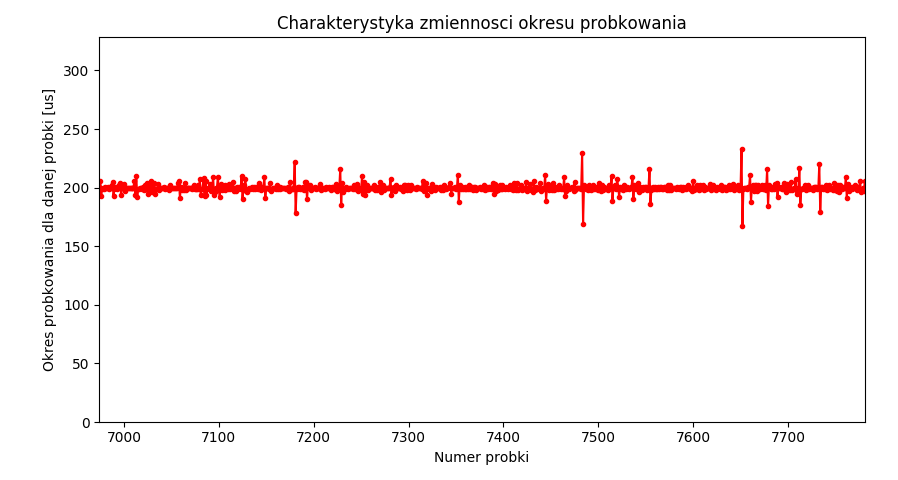
\includegraphics[width=14cm]{zmiennosc_probkowania_max1202}
	\caption{Charakterystyka zmienności okresu próbkowania przy użyciu sterownika do ADC} 
	\label{fig:zmiennosc_probkowania_max1202}
\end{figure}

Zmienność okresu próbkowania opisano przy użyciu parametru odchylenia standardowego. Wyniki z pomiaru napięcia sinusoidalnego w Tablicy 5.1.:

\begin{table}[t]
\label{tab5.1}
\centering
\begin{tabular}{|l|l|l|}
  \hline 
  Ilość zebranych próbek & 19958 \\
  \hline
  Średni okres próbkowania [$\mu$s] & 200 \\
  \hline
  Średnia częstotliwość próbkowania [Hz]& 5000 \\
  \hline 
  Wariancja okresu próbkowania [$\mu$s]  & 454 \\
  \hline
  Odchylenie standardowe okresu próbkowania [$\mu$s] & 21,3 \\
  \hline

  
\end{tabular}
\caption{Parametry opisujące zmienność okresu próbkowania} 
\end{table}


\subsubsection{Pomiar napięcia prostokątnego}

Wykonano również pomiar napięcia prostokątnego. Sygnał spróbkowano z częstotliwością 5kHz, charakterystyka jest przedstawiona na Rys. \ref{fig:rect_max1202_100Hz_adc}, a oscylogram na Rys. \ref{fig:rect_max1202_100Hz_osc} 

\begin{figure}[h]
	\centering
		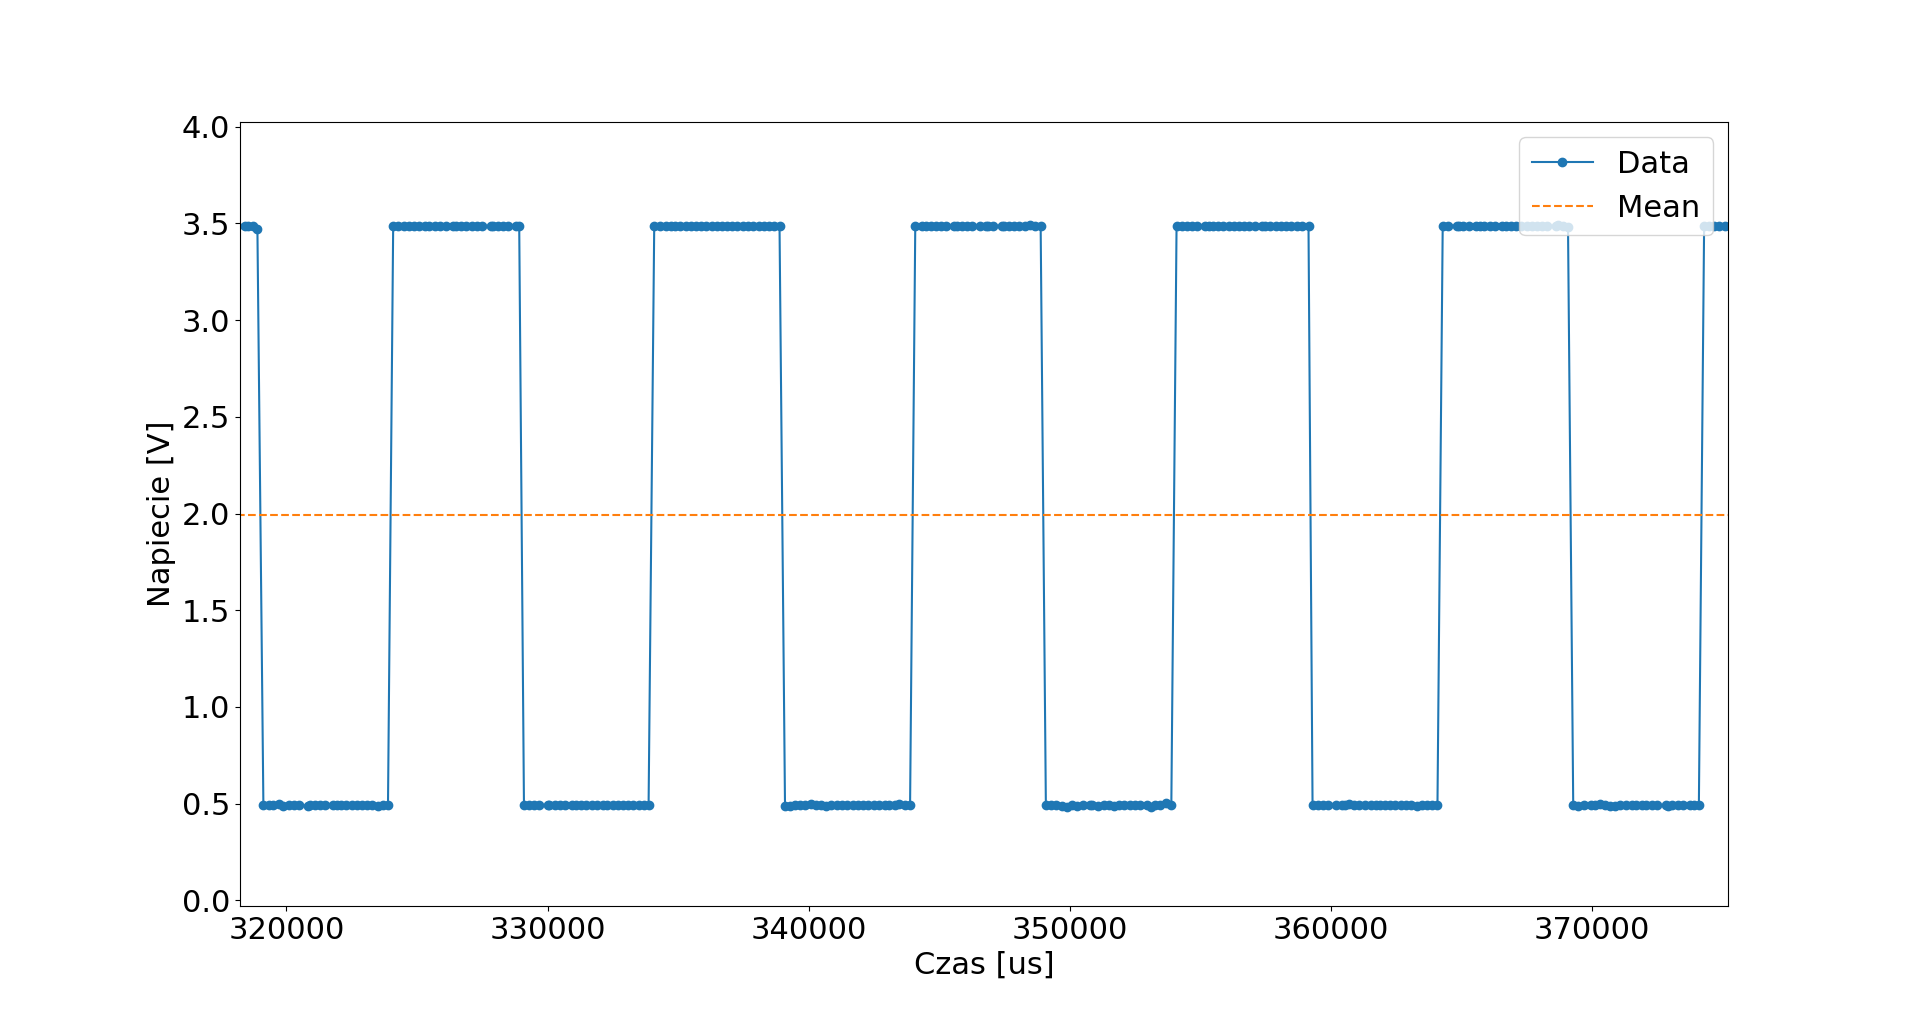
\includegraphics[width=15cm]{rect_max1202_100Hz_adc}
	\caption{Przebieg napięcia spróbkowanego przetwornika ADC MAX1202} 
	\label{fig:rect_max1202_100Hz_adc}
\end{figure}


\begin{figure}[h]
	\centering
		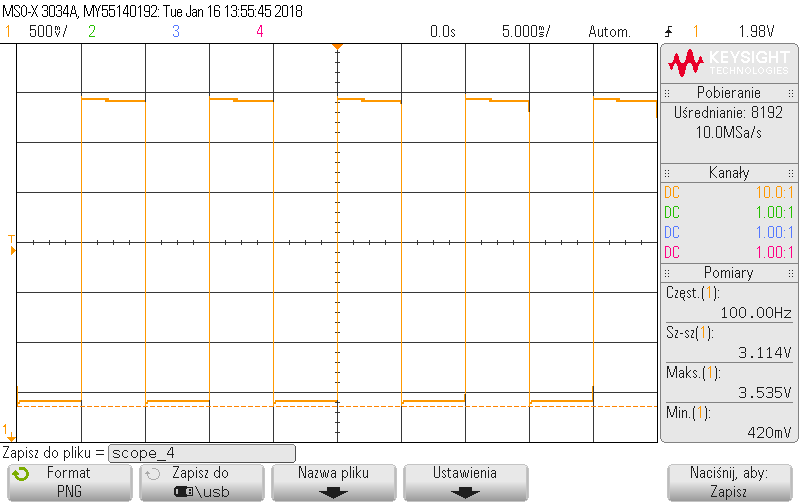
\includegraphics[width=12cm]{rect_max1202_100Hz_osc}
	\caption{Przebieg napięcia prostokątnego na oscyloskopie} 
	\label{fig:rect_max1202_100Hz_osc}
\end{figure}

\subsection{Analiza FFT sygnału sinusoidalnego}

Przed wykonaniem pomiaru dokonano symulacji komputerowej w celu dostrzeżenia różnic charakterystyk częstotliwościowych między sygnałem sinusoidalnym bez zniekształceń, a sygnałem z nierównomiernymi odstępami czasowymi pomiędzy kolejnymi próbkami. 
Sygnał został wygenerowany numerycznie, a następnie zniekształcony poprzez dodanie do wektora czasu pseudolosowych wartości z zakresu od 0 do 50us. Rysunek \ref{fig:sin_fft_ideal} przedstawia przebieg czasowy sygnału zniekształconego, jego charakterystykę częstotliwościową oraz widmo sygnału sinusoidalnego bez zniekształceń. Charakterystyki wyznaczono przy użyciu algorytmu FFT i przemnożeniu przez okno Hanninga.

\begin{figure}[H]

	\centering
		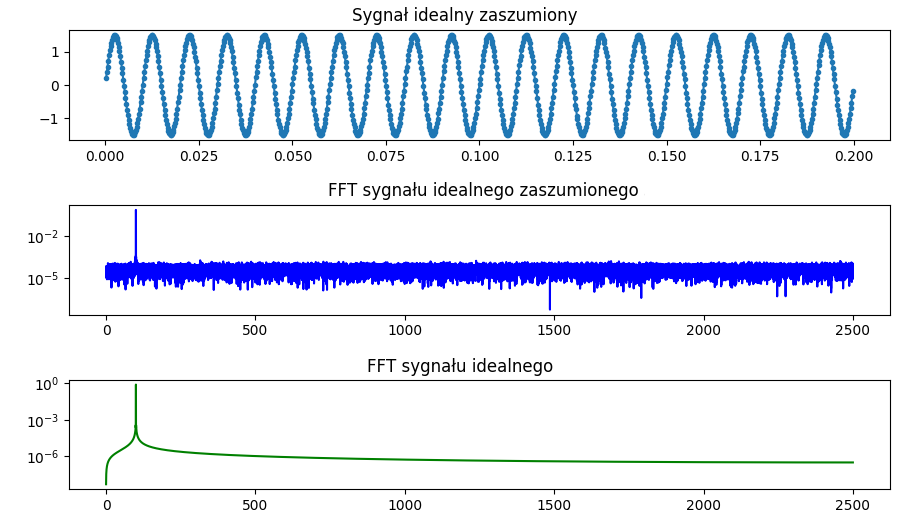
\includegraphics[width=14cm]{sin_fft_ideal}
	\caption{Analiza FFT dla sygnału sinus wygenerowanego numerycznie} 
	\label{fig:sin_fft_ideal}
\end{figure}

W celu zbadania stałości częstotliwości próbkowania przetwornika dokonano analizy FFT spróbkowanego sygnału. Rysunek \ref{fig:sin_fft_max1202} przedstawia przebieg czasowy otrzymany z 50000 próbek zebranych przetwornikiem ADC MAX1202, widmo sygnału spróbkowanego przemnożonego przez okno Hanning'a oraz charakterystyka częstotliwościowa sygnału sinusoidalnego wygenerowanego numerycznie.


\begin{figure}[H]
	%\centering
		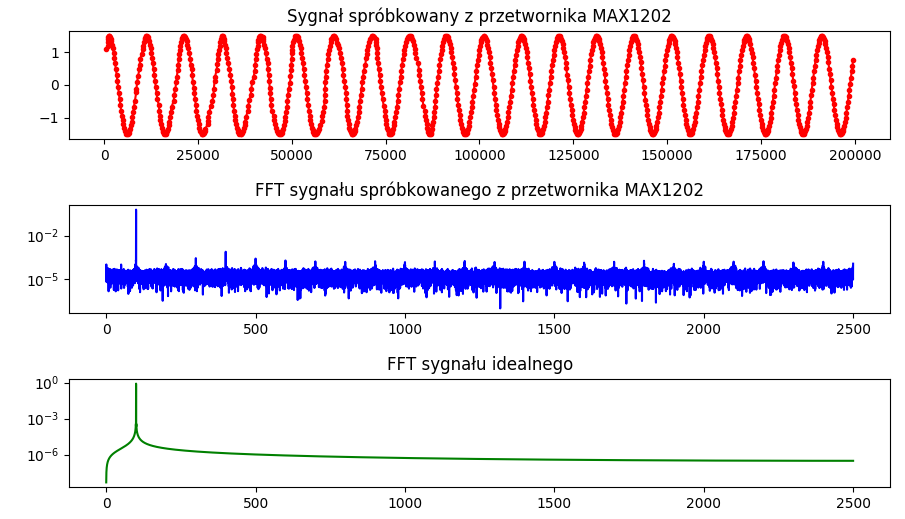
\includegraphics[width=14cm]{sin_fft_max1202}
	\caption{Analiza FFT dla sygnału spróbkowanego przetwornikiem ADC MAX1202} 
	\label{fig:sin_fft_max1202}
\end{figure}

\subsection{Pomiary ciśnienia czujnikiem LPS25H}

Zmierzono ciśnienie atmosferyczne w windzie gmachu Elektroniki i Technik Informacyjnych poruszającej się pomiędzy piętrami -2. i 4. zatrzymując się po drodze na 2. piętrze i na parterze. Na Rys. \ref{fig:winda} przedstawiono wyniki pomiarów. Jak widać na rysunku ciśnienie maleje zgodnie z wzorem barometrycznym wraz ze wzrostem wysokości. Po odpowiedniej kalibracji czujnik można wykorzystać do pomiaru wysokości.


\begin{figure}[H]
	\centering
		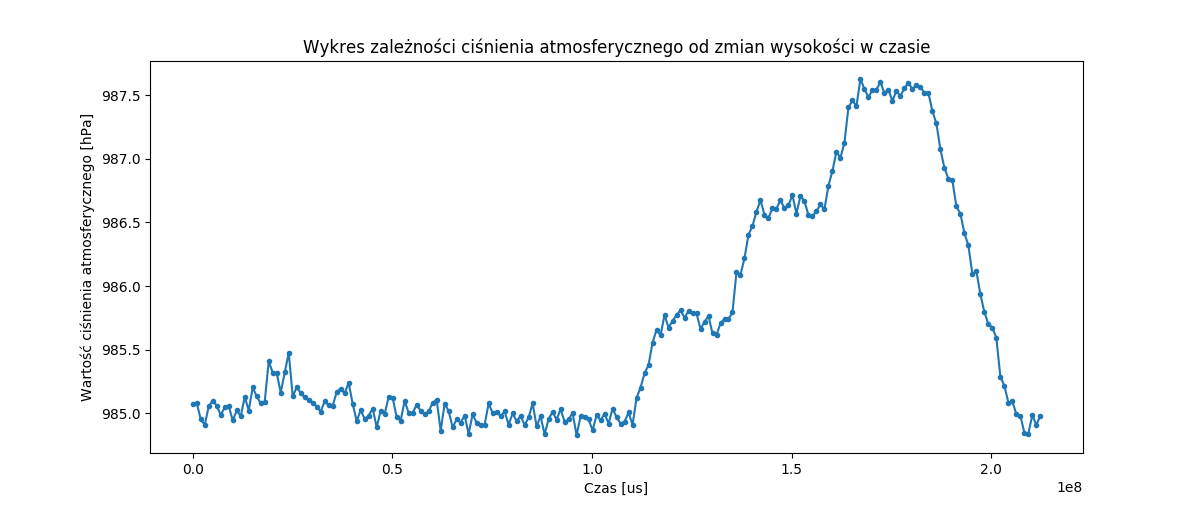
\includegraphics[width=14cm]{winda}
	\caption{Wykres zmian ciśnienia panującego w poruszającej się windzie} 
	\label{fig:winda}
\end{figure}


\section{Analiza wyników}
W celu dokonania porównania pomiaru maksymalnej częstotliwości próbkowania przeprowadzono analizę częstotliwościową spróbkowanego sygnału przy użyciu algorytmu FFT.
Zmienność częstotliwości próbkowania zobrazowano przy pomocy parametru odchylenia standardowego z poszczególnych odstępów czasowych pomiędzy momentami zebrania kolejnych próbek.

\begin{equation}
\sigma=\sqrt{\dfrac{1}{N}\sum_{0}^{N}{Var(x)}}
\end{equation}

x - odstępy pomiędzy momentami zebraniem próbki

N - ilość zebranych próbek


\subsection{Prezentacja i wizualizacja danych pomiarowych}
Optymalnym do tego zadania i znacznie ułatwiającym analizę wyników narzędziem był pakiet Pythona matplotlib. Są to pakiety zapewniające interfejs pozwalający na prezentację wyników w formie ułatwiającej analizę danych. Pliki z danymi ładowane były do aplikacji wyświetlającej wykresy w formacie pliku rozdzielanego przecinkami (csv).  




\chapter{Podsumowanie}
\label{ch:podsumowanie}


Cel pracy został osiągnięty, stworzono projekt i oprogramowanie sieciowego systemu akwizycji danych. Założenie optymalizacji kosztu zostało spełnione, układ jest dużo tańszy od rozwiązań komercyjnych, które najczęściej wymagają wykupienia licencji na oprogramowanie pozwalające sterowanie pomiarami. Główną część systemu - Raspberry Pi w wersji Zero W z modułem Wifi i Bluetooth 4.1 można nabyć za około 50zł.

Użytkownik komunikuje się z systemem dzięki interfejsowi graficznemu aplikacji w przeglądarce internetowej. Zaletą systemu jest jego łatwa rozszerzalność. Dokonanie niewielkich zmian w oprogramowaniu i możliwość podłączenia urządzeń do magistrali SPI i I2C oraz pozostałych pinów GPIO sprawia, że użytkownik jest w stanie rozszerzać system o nowe funkcjonalności. Ponadto fakt, iż Raspberry Pi jest popularnym minikomputerem w swojej dziedzinie, zapewnia użytkownikowi wsparcie w dokonywaniu ewentualnych zmian w konfiguracji i strukturze systemu akwizycji danych. 

Projekt może być użyty do zastosowań akwizycji danych, na przykład jako stacja meteorologiczna z możliwością zdalnego dostępu dzięki komunikacji sieciowej. Rozwiązania zawarte w projekcie umożliwiają podgląd danych w trakcie wykonywania pomiaru oraz pobranie danych przez użytkownika w celu wykonania dokładniejszej analizy. Część pracy zostanie wykorzystana podczas misji balonowej Studenckiego Koła Inżynierii Kosmicznej Politechniki Warszawskiej do zbierania danych z czujników udostępnianych przez łącze radiowe w paśmie radioamatorskim.

\begin{thebibliography}{9}


\bibitem{NI_6008}
National Instruments website, 

http://www.ni.com/en-us/support/model.usb-6008.html

\bibitem{AnalogDiscoveryDoc}
Analog Discovery 2 Reference Manual, 

https://reference.digilentinc.com/reference/instrumentation/

analog-discovery-2/reference-manual?redirect=1

\bibitem{raspfoundation}
Raspberry Pi Learning Resources, Raspberry Pi Software Guide, 

Raspberry Pi Foundation, 2017, 

https://www.raspberrypi.org/learning/software-guide/quickstart/

\bibitem{rpispecs}
Raspberry Pi – Wikipedia, Parametry techniczne platformy Raspberry Pi,

https://pl.wikipedia.org/wiki/Raspberry\_Pi

\bibitem{maxdatasheet}
ADC MAX1202 datasheet, 

https://datasheets.maximintegrated.com/en/ds/MAX1202-MAX1203.pdf

\bibitem{ntp}
Building a Raspberry-Pi NTP Server, 

http://raspberrypi.tomasgreno.cz/ntp-client-and-server.html

\bibitem{spidev}
SPI driver - spidev documantation

https://www.kernel.org/doc/Documentation/spi/spidev

\bibitem{i2cdev}
I2C driver - i2c-dev documantation

https://www.kernel.org/doc/Documentation/i2c/dev-interface

\bibitem{spiKernel}
Serial Peripheral Interface (SPI) — The Linux Kernel documentation, 

https://www.kernel.org/doc/html/v4.14/driver-api/spi.html

\bibitem{buildroot}
The Buildroot user manual, 2017, 

https://buildroot.org/downloads/manual/manual.html

\bibitem{paho.mqtt}
paho-mqtt 1.1 : Python Package Index

https://pypi.python.org/pypi/paho-mqtt/1.1

\bibitem{watchdog}
Watchdog install on Raspbian Jessie - Raspberry Pi Forums, 2017, 

https://www.raspberrypi.org/forums/viewtopic.php?t=175432


\end{thebibliography}


%\listoftodos[Notes]

\end{document}